
\documentclass[10pt]{article}
\usepackage{NotesTeXV3,lipsum}
\usepackage{cancel}
\usepackage{pgfplots}
\usepackage{esint}
\usepackage{listings}
\usepackage[table]{xcolor}% http://ctan.org/pkg/xcolor
\usetikzlibrary{shadows}
\usetikzlibrary{shapes}
\usetikzlibrary{decorations}
\usetikzlibrary{arrows,decorations.markings}
\usetikzlibrary{arrows,shapes.gates.logic.US,shapes.gates.logic.IEC,calc}
\pgfplotsset{compat=newest}
\usepgfplotslibrary{colormaps}
% \usepackage{showframe}
% http://tex.stackexchange.com/q/169557/5764
\usepackage{mathtools}
\usepackage{circuitikz}
\DeclarePairedDelimiter{\norm}{\lVert}{\rVert}
\newcommand{\vectorproj}[2][]{\text{proj}_{\vect{#1}}\vect{#2}}
\newcommand{\vect}{\mathbf}
\usepackage{circuitikz}
\usepackage{longdivision}

% The following are to allow Multiplication, addition and long division written out.
% See https://tex.stackexchange.com/questions/169842/how-to-make-a-multiply-equation
\usepackage{array}

\makeatletter
\pgfdeclareshape{custom multiplexer}{
  \expandafter\pgfutil@g@addto@macro\csname pgf@sh@s@custom multiplexer\endcsname{%
    % Adjust the height based on the number of inputs
    \pgfmathsetmacro{\muxheight}{\pgfkeysvalueof{/pgf/minimum height} - (\pgfkeysvalueof{/pgf/inner ysep} * 2)}
    \pgfpathrectanglecorners{\pgfpoint{-0.5\wd\pgfnodeparttextbox}{-0.5\muxheight}}{\pgfpoint{0.5\wd\pgfnodeparttextbox}{0.5\muxheight}}
  }
}

    \providecommand\text\mbox
    \newenvironment{arithmetic}[1][]{\begin{tabular}[#1]{Al}}{\end{tabular}}
    \newcolumntype{A}{>{\bgroup\def~{\phantom{0}}$\@testOptor}r<{\@gobble\\$\egroup}}

\def\@testOptor\ignorespaces#1#2\\{%
    \ifx#1\times
        \@OperatorRow{#1}{#2}\@tempa%
    \else\ifx#1+
        \@OperatorRow+{#2}\@tempa%
    \else\ifx#1\discretionary% detects the soft hyphen, \-
        \@ShortSubtractRow{#2}\@tempa%
    \else\ifx#1-
        \@OperatorRow-{#2}\@tempa%
    \else
        \@NormalRow{#1#2}\@tempa%
    \fi\fi\fi\fi
    \@tempa}

\def\@OperatorRow#1#2#3{%
    \@IfEndRow#2\@gobble\\{%
        \def#3{\underline{{}#1 #2}\\}%
    }{%
        \def#3{\underline{{}#1 #2{}}}%
    }}

\def\@NormalRow#1#2{%
    \@IfEndRow#1\@gobble\\{%
        \def#2{#1\\}%
    }{%
        \def#2{#1{}}%
    }}

\def\@IfEndRow#1\@gobble#2\\#3#4{%
    \ifx#2\@gobble
        #4%
    \else
        #3%
    \fi}

  \makeatother

\def\@ShortSubtractRow#1#2{\@@ShortSubtractRow#1~\end{#2}}
\def\@@ShortSubtractRow#1#2~#3\end#4{%
    \@IfEndRow#3\@gobble\\{%
        \def#4{\underline{\text{--} #2}#3\\}%
    }{%
        \def#4{\underline{\text{--} #2{}}#3}%
      }}

\def\Into#1\\{%
    \@IfEndRow#1\@gobble\\{%
        \def\@tempa{~\raisebox{0.17ex}{\parbox{0.15em}{\centering$\big|$}}\overline{~\big.#1}\\}%
    }{%
        \def\@tempa{~\raisebox{0.17ex}{\parbox{0.15em}{\centering$\big|$}}\overline{~\big.#1{}}}%
      }\@tempa}

\usepackage{colortbl}

\begin{document}
	\title{{CS10 -- Computer Architecture and Organization}\\{\normalsize{\itshape My Notes}}}
	\author{Leonard Mohr}
	\affiliation{
	Student at Foothill College
	}
	\emailAdd{leonardmohr@gmail.com}
	\maketitle
	\newpage
	\pagestyle{fancy}

\section{Computer Abstractions and Technology}
\subsection{Introduction}\label{subsec:}
\begin{figure}[H]
  \centering
  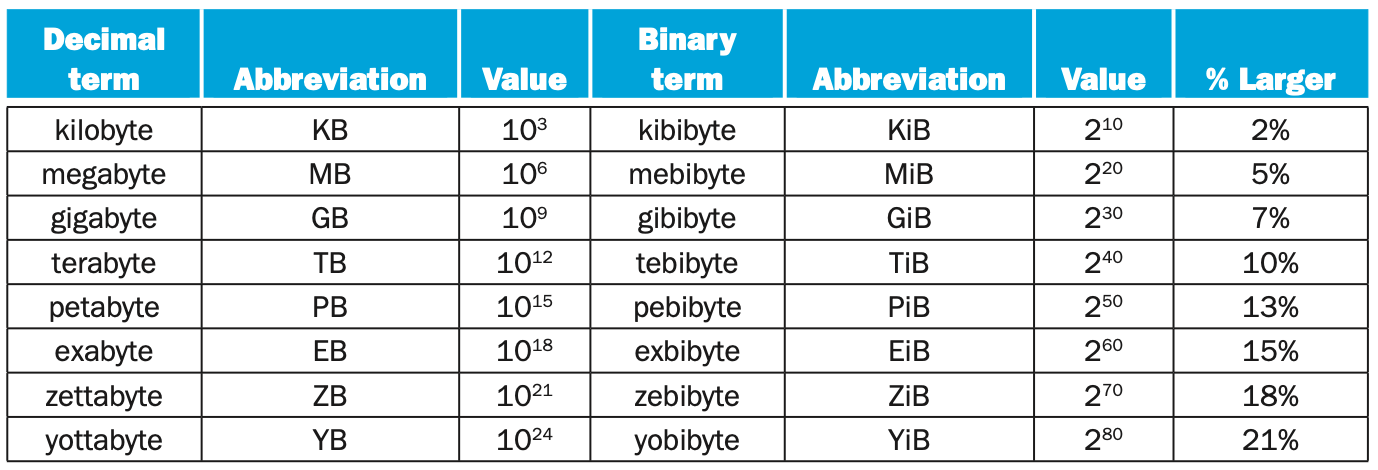
\includegraphics[width=11cm]{1.png}
  \caption{We can describe storage in binary or decimal notation. We are much more familiar with the decimal term.  Note also the size difference between the two: binary term gets progressivly larger.}
  \label{fig:}
\end{figure}

\subsubsection{Program Performance}
One of the main goals for both the hardware designer and the software designer is to improve performance.  This can be achieved in different ways (just think about how quick sort is much faster than bubble sort, and the apple M1 processor is much faster than the intel processors they replaced).
\begin{figure}[H]
  \centering
  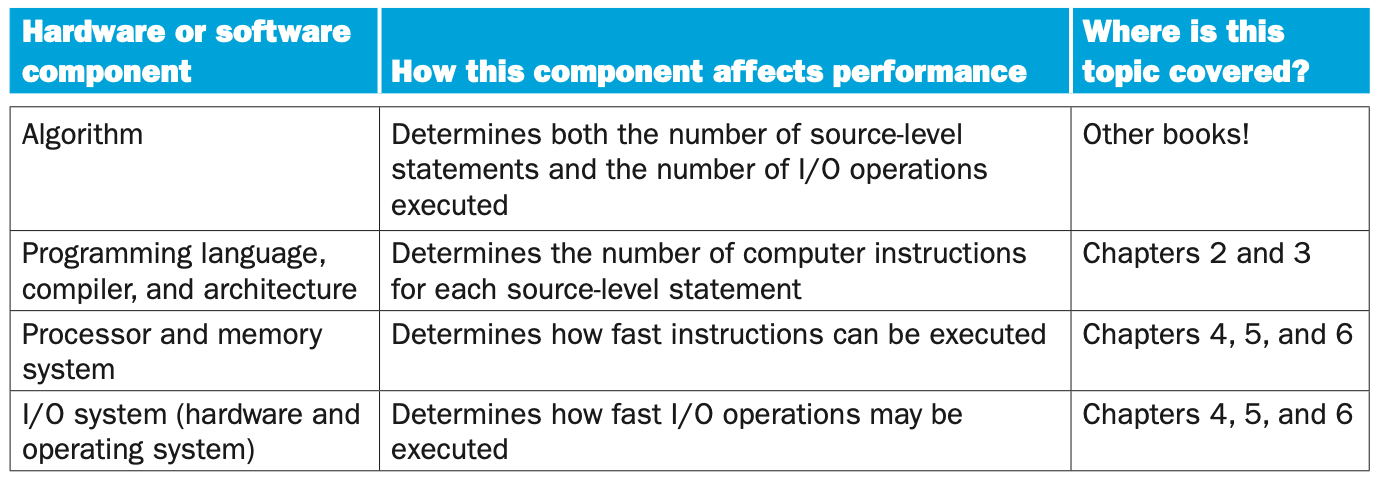
\includegraphics[width=11cm]{2.png}
  \caption{Here we can see the various ways program performance can be improved.}
  \label{fig:}
\end{figure}

\textbf{Check Yourself}
\begin{enumerate}
\item As mentioned earlier, both the software and hardware affect the performance of a program. Can you think of examples where each of the following is the right place to look for a performance bottleneck?
\begin{enumerate}[label=\alph*)]
\item The algorithm chosen
  \begin{tcolorbox}[%
    enhanced, 
    breakable,
    frame hidden,
    overlay broken = {
      
      (frame.north west) rectangle (frame.south east);},
    ]
If a program that sorts a really long list of names is taking a long time, you might want to look at the algorithm being used.
\end{tcolorbox}
\item The programming language or compiler
  \begin{tcolorbox}[%
    enhanced, 
    breakable,
    frame hidden,
    overlay broken = {
      
      (frame.north west) rectangle (frame.south east);},
    ]
If your program could is not language dependent, you could look at using a compiled language (like C), as opposed to an interpreted language like Python.
\end{tcolorbox}
\item The operating system
  \begin{tcolorbox}[%
    enhanced, 
    breakable,
    frame hidden,
    overlay broken = {
      
      (frame.north west) rectangle (frame.south east);},
    ]
If one program runs well, but two at a time don't, then maybe the operating system isn't distributing it's resources efficiently.
\end{tcolorbox}
\item The processor
  \begin{tcolorbox}[%
    enhanced, 
    breakable,
    frame hidden,
    overlay broken = {
      
      (frame.north west) rectangle (frame.south east);},
    ]
If the computer in general is using a lot of energy, you might want to look at the processor. Similarily, if you are doing compute heavy tasks such as vdeo editing, you might need a processor upgrade.
\end{tcolorbox}

\item The I/O system and devices
  \begin{tcolorbox}[%
    enhanced, 
    breakable,
    frame hidden,
    overlay broken = {
      
      (frame.north west) rectangle (frame.south east);},
    ]
If it takes a long time to write to a hard drive, you might look at upgrading to a SSD.
  \end{tcolorbox}
\end{enumerate}
\end{enumerate}

\subsection{Eight Great Ideas in Computer Architecture}\label{subsec:}
\begin{enumerate}
\item \textbf{Moore's Law}\\
  Moore's Law resulted from a 1965 prediction that integrated circuit (IC) resources would double every 18-24 months.
\begin{marginfigure}
  \begin{center}
    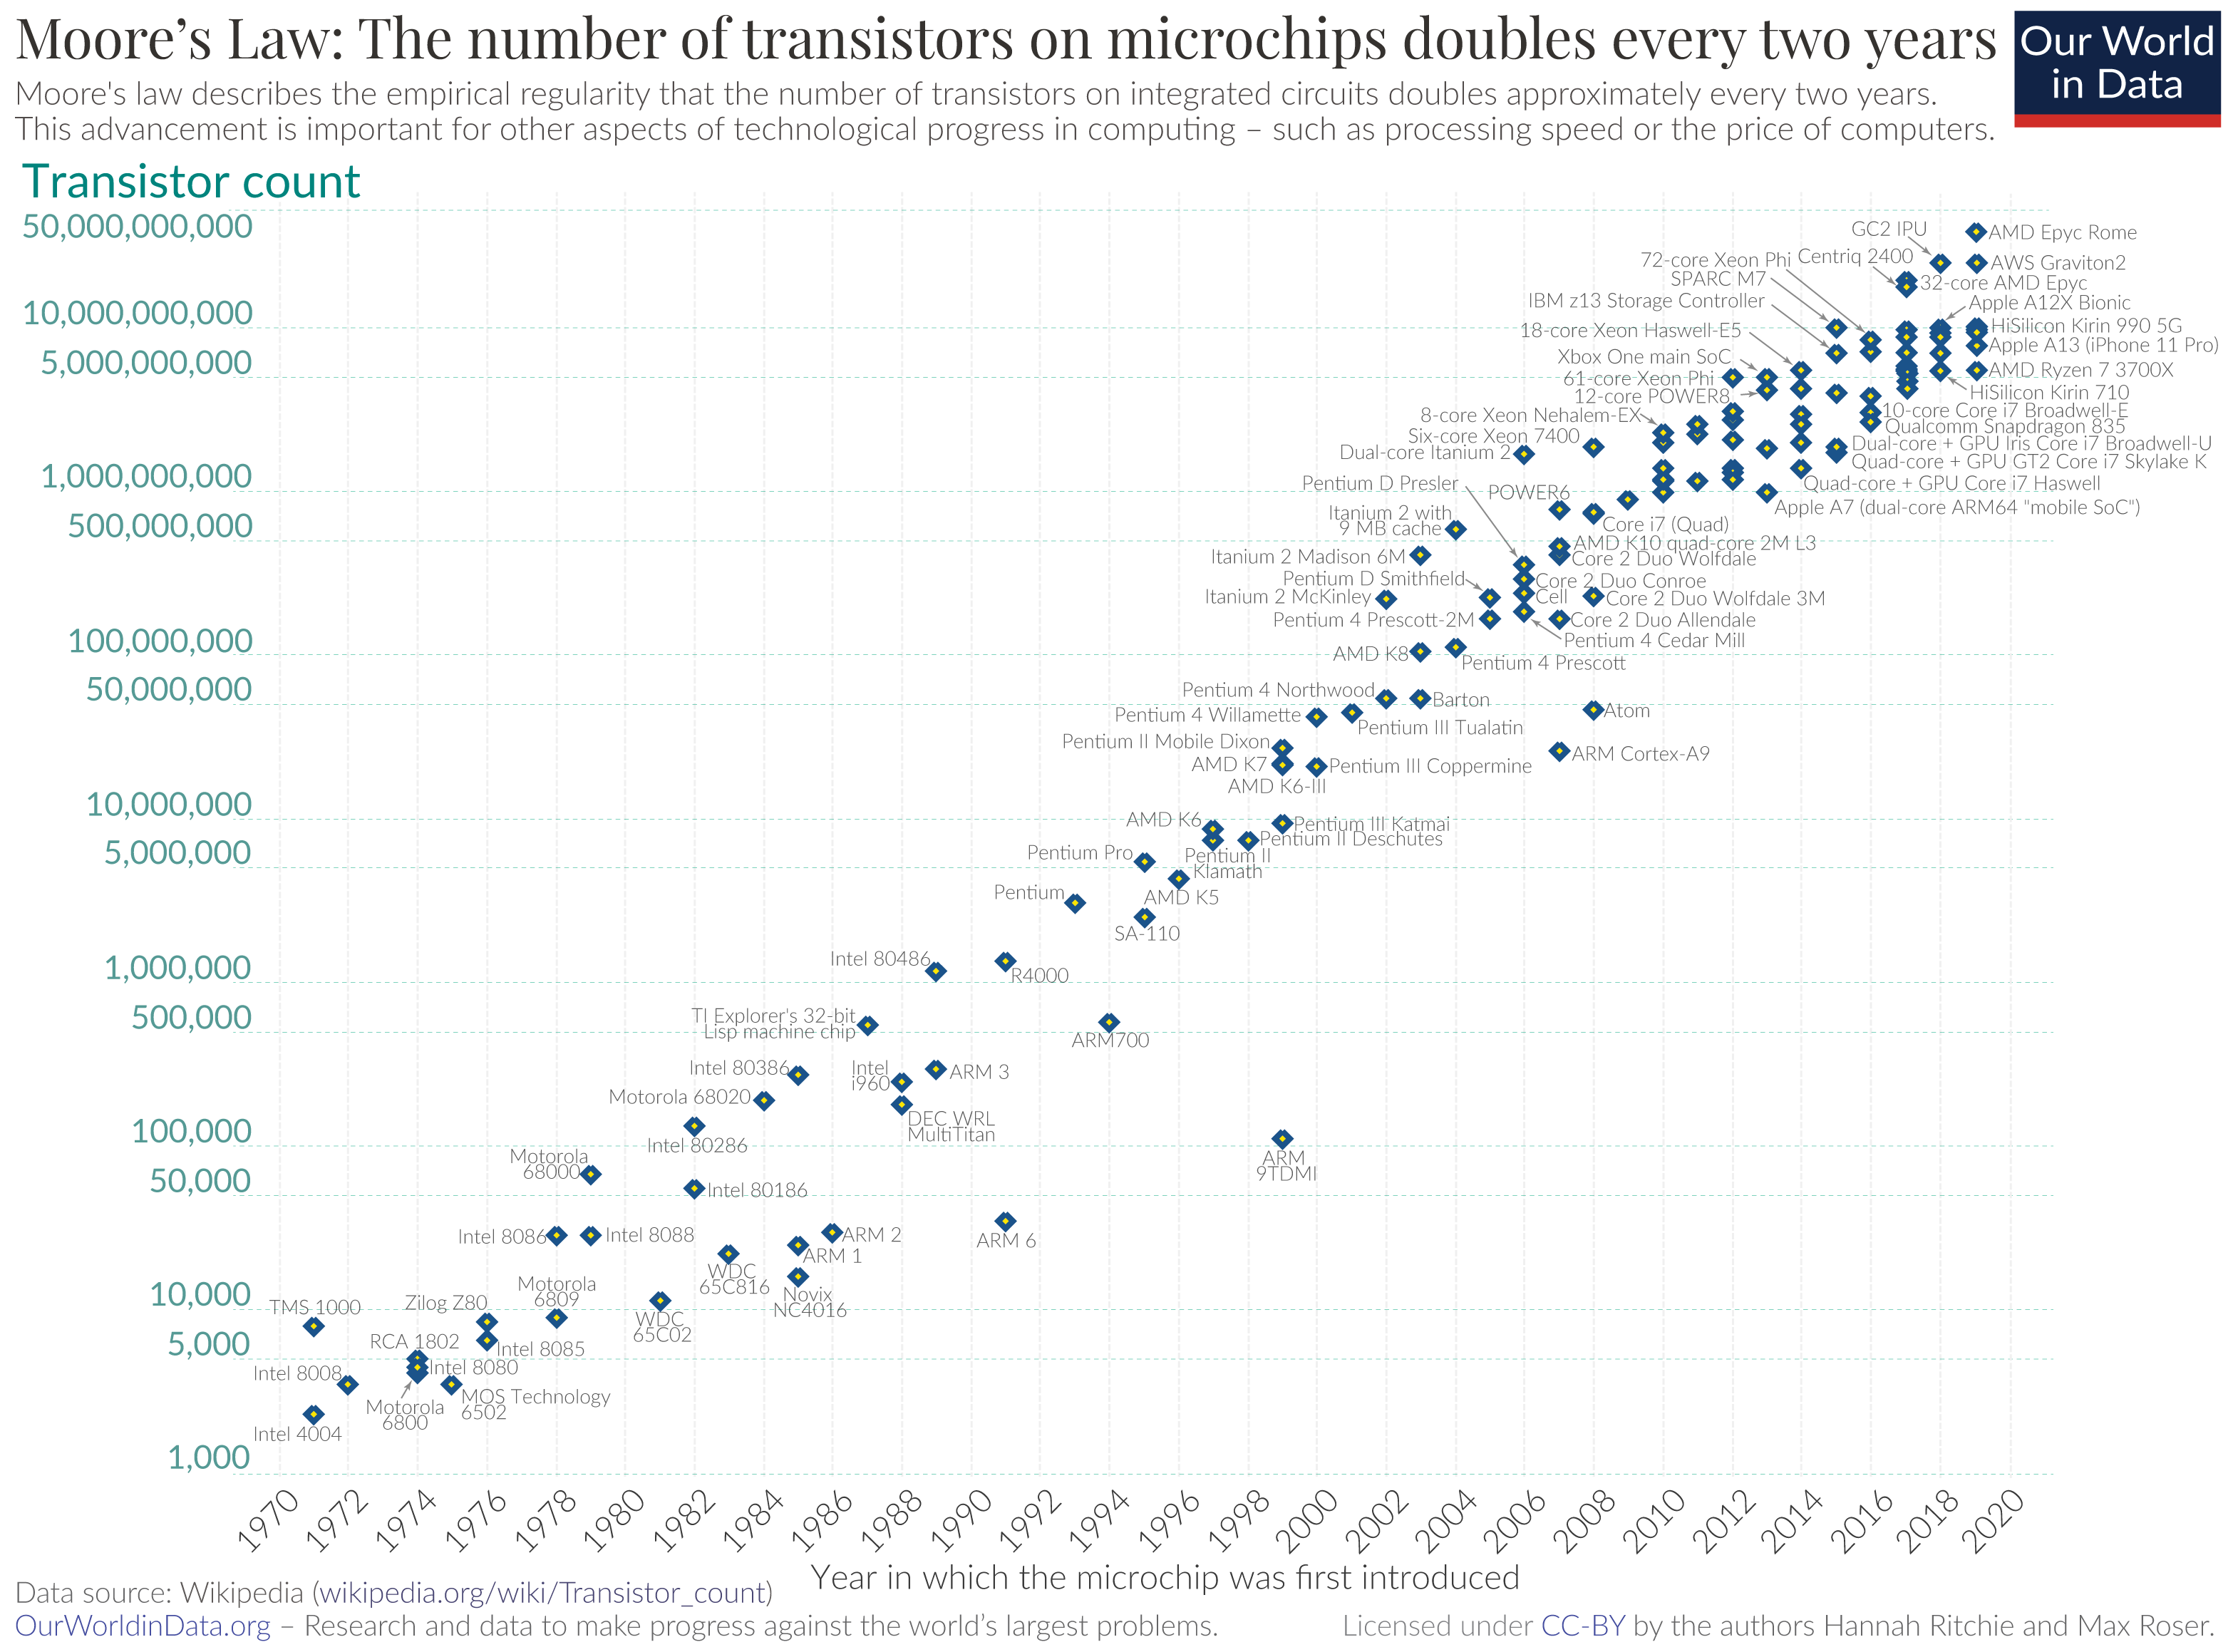
\includegraphics[width=\linewidth]{3.png}
  \end{center}
  \caption{Moore's Law in action.}
\end{marginfigure}%

\item \textbf{Use Abstraction to Simplify Design}\\
  To increase productivity, by design both computer architects and programmers try use abstractions to hide the lower-level details and provide a simpler to work with.  For example, the operating system abstracts away the complexity of the memory system so that programs are provided with a much simplified view of the memory, and the details are handled by the operating system.

\item \textbf{Make the Common Case Fast}\\
  Better performance gains can be made if you optimize for what the prgram is going to do most often.
\item \textbf{Performance via Parallelism}\\
  We can make a program a lot faster by performing multiple tasks at once.  This is especially true with the advent of multi-core processors.
\item \textbf{Performance via Pipelining}\\
  If you are moving a lot of bricks from one place to another (using just manpower) it would be a lot more efficient to set up a line of people, and pass the bricks down the line, than to just have everyone running back and forth.  The same principle can be used in computers.

\item \textbf{Performance via Prediction}\\
  When a processor encounters an if statement, it might say that on average the result is true, and procede like it is, so that it keep going, and then the if qualifier can be processed at a later date.

\item \textbf{Hierarchy of Memories}\\
  By using different types of memory, from really small and really fast, to really large and slow, a memory hierarchy is created.  Caches give the programmer the illusion that main memory is nearly as fast as the top of the hierarchy and nearly as big and cheap as the bottom of the hierarchy.

\item \textbf{Dependability via Redundancy}\\
Because we are sad when a computer dies, we want to prevent the death of the computer.  To do this we make them dependable.  This can be achieved by including redundant components that can both take over in the event of a failure as well as detect when a failure has occured.
\end{enumerate}

\subsection{Below Your Program}\label{subsec:}
The Operating System is a great example of abstraction.  Some of its most important functions are:
\begin{itemize}
\item Handling basic input and output operations
\item Allocating storage and memory
\item Provided for protected sharing of the computer among multiple applications using it simultaneously.
\end{itemize}
Another example of abstraction is high-level programming languages like C.  When computers first came about, programmers programmed in binary; they wrote their programs in $1$'s and $0$'s (the language of the computer).  Since that was tedious, they invented the assembler which would convert assembly language into binary code.  Next came the compiler which would convert higher order languages into assembly.

Another benefit of the programming languages is it allows one to chose the specific language that is best for the task.  Also, programs don't have to be written for a specific processor, since the compiler and assembler can package it for different computers.

\subsection{Under the Covers}\label{subsec:}
The five classic components of a computer are input, output, memory, datapath, and control, with the last two sometimes combined and called the processor. This organization is independent of hardware technology: you can place every piece of every computer, past and present, into one of these five categories.
\begin{marginfigure}
  \begin{center}
    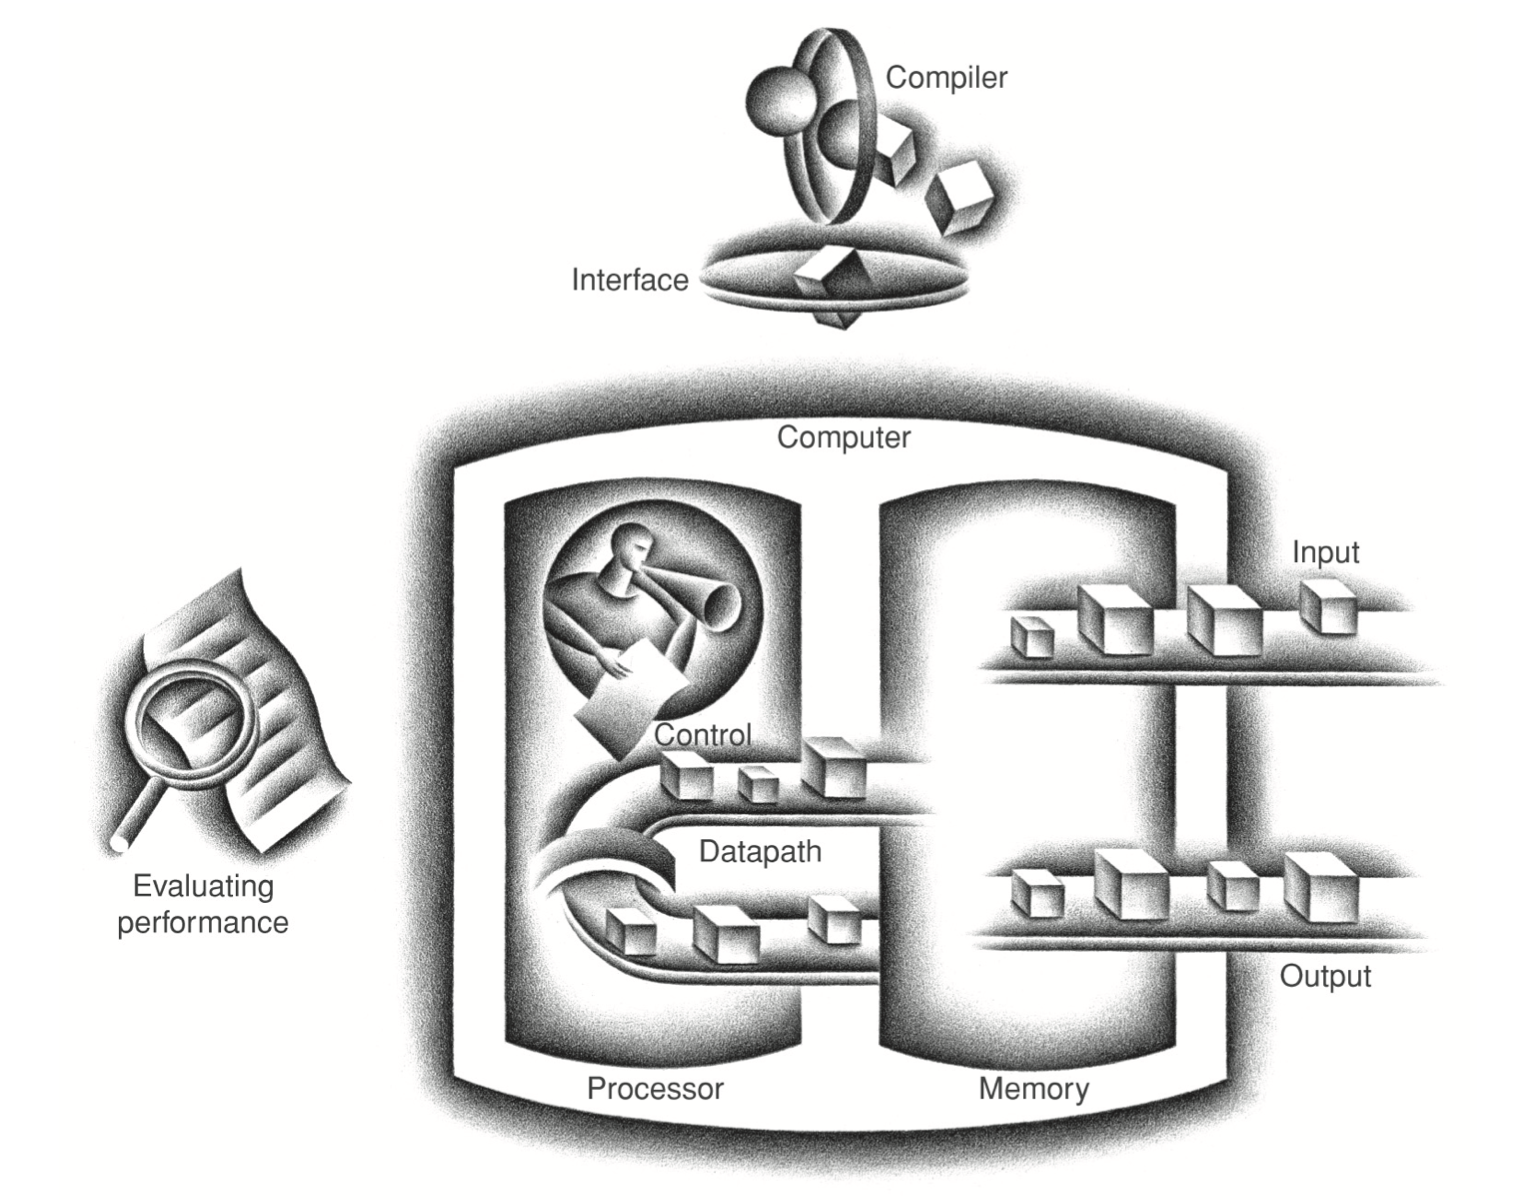
\includegraphics[width=\linewidth]{4.png}
  \end{center}
  \caption{Here we see the flow of information in a computer.  The processor gets instructions and data from memory. Input writes data to memory, and output reads data from memory.  Control sends the signals that determine the operations of the datapath, memory, input, and output.}
\end{marginfigure}%
\subsubsection{Parts of the Computer}
\begin{itemize}
\item Integrated Circuit: Also called a chip. A device combining dozens to millions of transistors.
\item Central Processing Unit (CPU): Also called the processor. The active part of the computer, which contains the datapath and control and which adds numbers, tests numbers, signals I/O devices to activate, and so on.
\item Datapath: The component of the processor that performs arithmetic operations
\item Control: The component of the processor that commands the datapath, memory, and I/O devices according to the instructions of the program.
\item Memory: The storage area in which programs are kept when they are running and that contains the data needed by the running programs.
\item Dynamic Random Access Memory (DRAM): Memory built as an integrated circuit; it provides random access to any location Access times are 50 nanoseconds and cost per gigabyte in 2012 was $\$5$ to $\$10$.
\item Cache Memory: Consists of a small, fast memory that acts as a buffer for the DRAM memory.
\item Static Random Access Memory: SRAM is faster but less dense, and hence more expensive, than DRAM.
\item Instruction Set Architector: The interface between the hardware and the lowest-level software.  This includes all the information necessary to write a machine language program that will run correctly, including instructions, registers, memory access, I/O, and so on.
\item Application Binary Interface (ABI): The user portion of the instruction set plus the operating system interfaces used by application programmers. It defines a standard for binary portability across computers. 
\end{itemize}
\addtocounter{subsection}{1}
\subsection{Performance}\label{subsec:}
When talking about computers, we often want to look at the performance of the computer.  But how can we define performance?
\begin{definition}
  \textbf{Response Time}\\
  Also referred to as \textbf{execution time}.  This is the total time required for the computer to complete a task, including disk access, memory aaccesses, I/O activities, operating system overhead, CPU execution time, and so on.
\end{definition}
\begin{definition}
  \textbf{Throughput / Bandwidth}\\
  This measures the number of tasks computed per unit time.
\end{definition}
For the time being, we will mostly be looking at response time.  So that a higher number represents a machine with better performance we will say that
\[\text { Performance }_{\mathrm{X}}=\frac{1}{\text { Execution time }_{\mathrm{X}}}.\]
Also, we often want to say that computer ``X is $n$ times as fast as Y'', to compute $n$ we say:
\[\frac{\text { Performance }_{\mathrm{X}}}{\text { Performance }_{\mathrm{Y}}} = \frac{\text{Execution Time}_Y }{\text{Execution Time}_X }=n.\]
\begin{marginfigure}
\textbf{CPU execution time} or simply \textbf{CPU time} is the actual time the CPU spends computing for a specific task.
\end{marginfigure}%
\subsubsection{Clock Rate and Clock Period}
Designers refer to the length of a \textbf{clock period} both as the time for a complete clock cycle (e.g., 250 picoseconds) and as the \textit{clock rate} (e.g., 4 gigahertz, or 4GHz), which is the inverse of the clock period.

For example a clock rate of
\begin{align*}
  4\text{GHz } &= 4,000,000,000 \frac{\text{cycles}}{\text{sec}}\\
               &\equiv \frac{1 \text{ cycle}}{4,000,000,000 \text{ second}}\\
               &= 0.00000000025 \frac{\text{cycle}}{\text{second}}\\
               &= \frac{1}{250} \frac{\text{cycle}}{\text{picosecond}}.
\end{align*}
We can relate clock cycles and clock cycle time to CPU time:
$$
\begin{aligned}
& \text { CPU execution time } \\
& \text { for a program }
\end{aligned}=\begin{aligned}
& \text { CPU clock cycles } \\
& \text { for a program }
\end{aligned} \times \text { Clock cycle time }
$$
or alternatively,
$$
\begin{aligned}
& \mathrm{CPU} \text { execution time } \\
& \text { for a program }
\end{aligned}=\frac{\mathrm{CPU} \text { clock cycles for a program }}{\text { Clock rate. }}
$$
\subsubsection{Instruction Performance}
In addition to thinking about clock cycles and CPU time, we also need to think about number of instructions there are in a program and the time each instruction takes:
\[\text{CPU clock cycles } = \text{ Instructions for a Program} \times \frac{\text{average clock cycles}}{\text{instruction}}\]
\begin{marginfigure}
\textbf{Clock Cycles per Instruction (CPI)} is the average number of clock cycles per instruction for a program or program fragement.
\end{marginfigure}%
\subsubsection{The Classic CPU Performance Equation}
Putting everything from above together we have
\[
\mathrm{CPU} \text { time }=\text { Instruction count } \times \mathrm{CPI} \times \text { Clock cycle time }
\]
and
\[\mathrm{CPU} \text { time }=\frac{\text { Instruction count } \times \mathrm{CPI}}{\text { Clock rate}}.\]
We also have
\[\text { Time }=\text { Seconds } / \text { Program }=\frac{\text { Instructions }}{\text { Program }} \times \frac{\text { Clock cycles }}{\text { Instruction }} \times \frac{\text { Seconds }}{\text { Clock cycle.}}\]
\begin{marginfigure}
Processors these days can vary their clock rates.  For example Intel Core i7 chips temporarily increase clock rate by $10\%$ until the chip gets too warm.  Thus we need to use the average clock rate for a program.
  \caption{}
\end{marginfigure}%
\addtocounter{subsection}{3}
\subsection{Fallacies and Pitfalls}\label{subsec:}
\subsubsection{Amdahl's Law}
\begin{definition}
  \textbf{Amdahl's Law}\\
  A rule stating that the performance enhancement possible with a given improvement is limited by the amount that the improved feature is used:
\begin{align*}
  \text{Execution time after improvement}
  &= \frac{\text{Execution time affected by improvement}}{\text{Amount of improvement}}\\
    &+ \text{ Execution time unaffected} 
\end{align*}
where Amount of improvement $= n$.
\end{definition}
We thus see that there is only so much benefit that can be achieved by improving a part of the program that is rarely used.  For this reason we want to make the common case fast!
\subsubsection{MIPS}
One should be wary about using only a subset of the performance equation as a performance metric; one can't determine performance just by looking at clock rate, instruction count, or CPI alone.\\\\
An alternative to time is \textbf{MIPS (million instructions per second)}:
\begin{align*}
\text{MIPS }&= \frac{\text{Instruction count}}{\text{Execution time } \times 10^6}.
\end{align*}
There are a couple problems with MIPS:
\begin{itemize}
\item MIPS specifies the instruction execution rate but does not take into account the capabilities of these instructions. Therefore we can't compare computers with different instruction sets.
\item MIPS varies between programs on the same computer; thus a computer cannot have a single MIPS rating.
\end{itemize}
\[\text { MIPS }=\frac{\text { Instruction count }}{\frac{\text { Instruction count } \times \text { CPI }}{\text { Clock rate }} \times 10^6}=\frac{\text { Clock rate }}{\mathrm{CPI} \times 10^6}.\]
\subsubsection{Check Yourself}
Consider the following performance measurements for a program:
\begin{center}
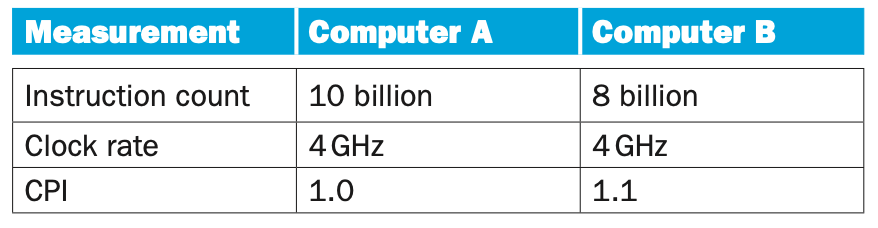
\includegraphics[width=6cm]{5.png}
\end{center}
Which computer is faster and which has the higher MIPS rating?
  \begin{tcolorbox}[%
    enhanced, 
    breakable,
    frame hidden,
    overlay broken = {
      
      (frame.north west) rectangle (frame.south east);},
    ]
    First looking at computer A.
\begin{align*}
  \text{ Time}(A) &= \frac{\text{CPU Clock Cycles} }{\text{Clock Rate} }\\
                  &= \frac{\text{Instruction Count }\times \text{ CPI}}{\text{Clock Rate}}\\
                  &= \frac{10 \times 10^9 \text{ instructions} \times \frac{1 \text{ cycle}}{\text{instruction}}}{4\times 10^9 \frac{\text{cycles}}{\text{second}}}\\
  &= 2.5 \text{ seconds}.
\end{align*}
\begin{align*}
  \text{MIPS}(A) &= \frac{\text{Instruction Count}}{\text{Execution Time } \times 10^6}\\
                 &= \frac{10 \times 10^9 \text{ instructions}}{2.5 \text{ seconds } \times 10^6}\\
                 &= \frac{4 \times 10^3 \text{ million instructions}}{\text{second}}.
\end{align*}
Now looking at computer B.
\begin{align*}
 \text{ Time}(B) &= \frac{\text{CPU Clock Cycles} }{\text{Clock Rate} }\\
                  &= \frac{\text{Instruction Count }\times \text{ CPI}}{\text{Clock Rate}}\\
                  &= \frac{8 \times 10^9 \text{ instructions} \times \frac{1.1 \text{ cycles}}{\text{instruction}}}{4\times 10^9 \frac{\text{cycles}}{\text{second}}}\\
  &= 2.2 \text{ seconds}.
\end{align*}
\begin{align*}
  \text{MIPS}(B) &= \frac{\text{Instruction Count}}{\text{Execution Time } \times 10^6}\\
                 &= \frac{8 \times 10^9 \text{ instructions}}{2.2 \text{ seconds } \times 10^6}\\
                 &\approx \frac{3.6 \times 10^3 \text{ million instructions}}{\text{second}}.
\end{align*}
We thus see that Computer A has a higher MIPS score but runs slower.
\end{tcolorbox}

\section{Instructions: Language of the Computer}
\addtocounter{subsection}{1}
\subsection{Operations of the Computer Hardware}\label{subsec:}
\subsubsection{MIPS Operands}
\begin{center}
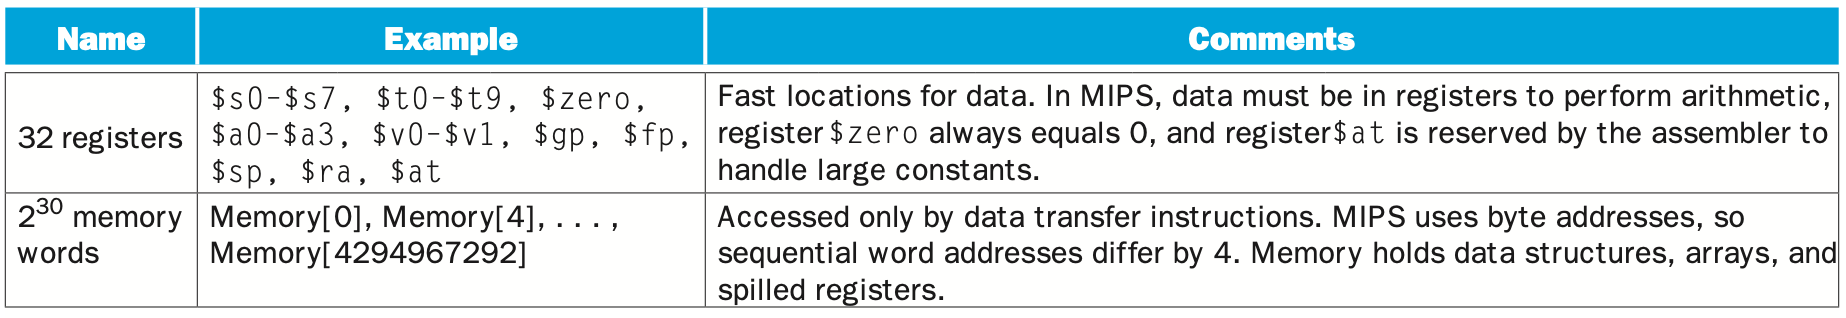
\includegraphics[width=\linewidth]{6.png}
\end{center}
\subsubsection{MIPS Instructions}
\begin{center}
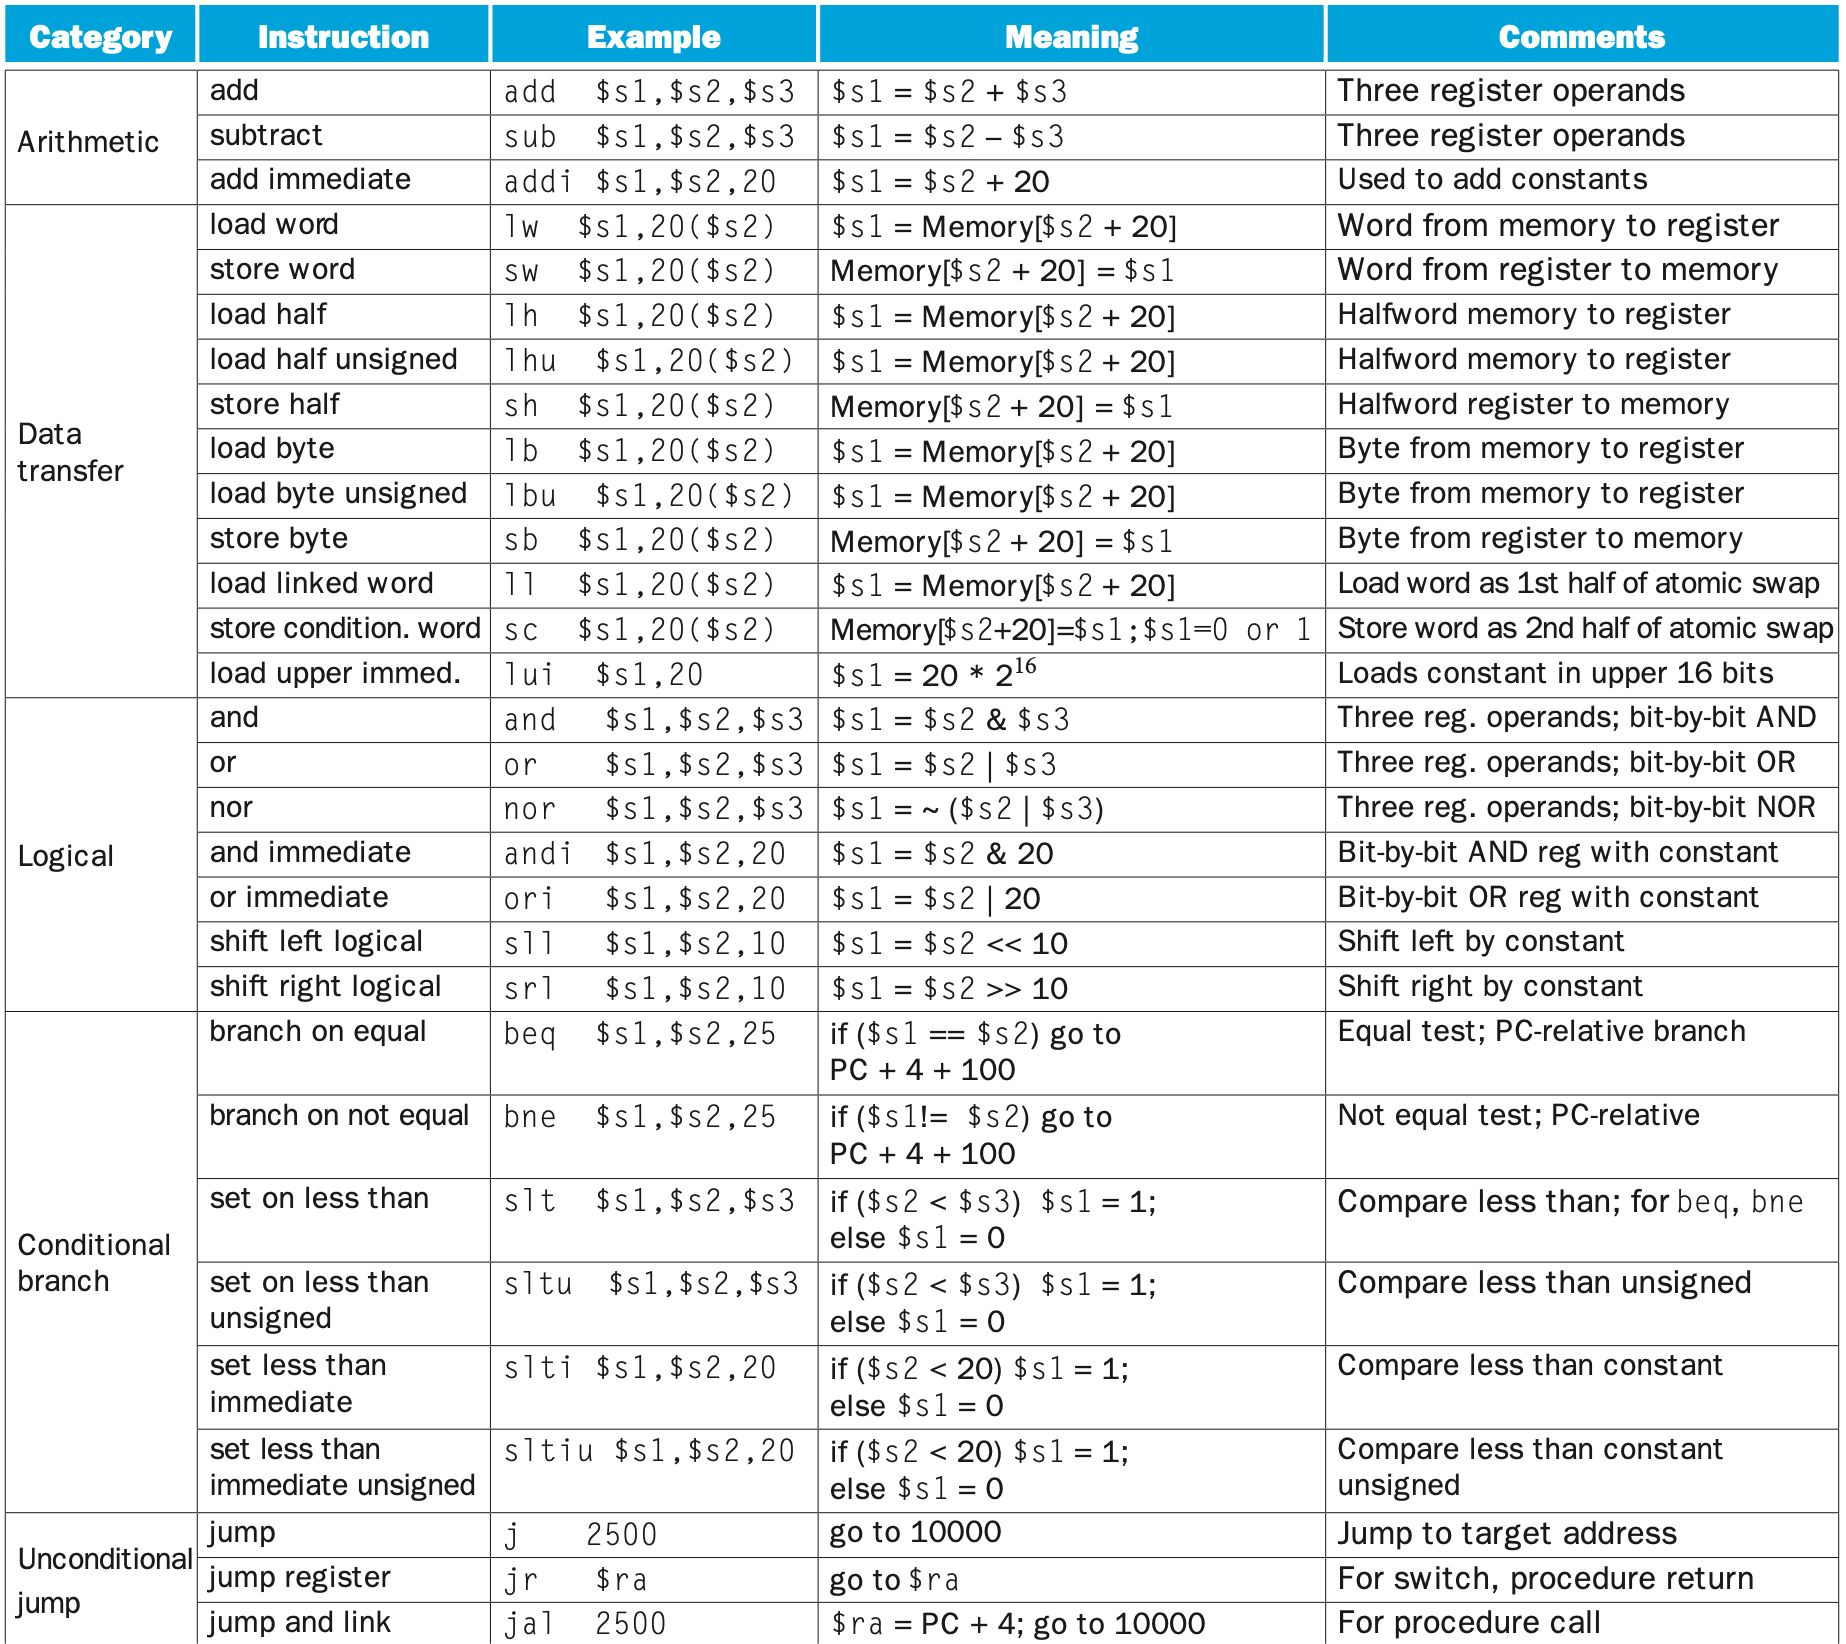
\includegraphics[width=\linewidth]{7.png}
\end{center}
Note how just about all operations have exactly three operands.  This conforms to the philosophy of keeping the hardware simple: hardware for a variable number of operands is more complicated than hardware for a fixed number.

\subsection{Operands of the Computer Hardware}\label{subsec:}
\subsubsection{Memory Operands}
Let's say we have the following C statement
\begin{lstlisting}[style=CStyle, numbers=left, xleftmargin=5.0ex, aboveskip=2em, belowskip=2em, numberstyle=\color{blue}, escapeinside=||]
g = h + A[8];
\end{lstlisting}
What will be the associated MIPS code if $g$ and $h$ are in registers $\$s1$ and $\$s2$, and that the base address of the array is in $\$s3$.
\begin{lstlisting}[style=CStyle, numbers=left, xleftmargin=5.0ex, aboveskip=2em, belowskip=2em, numberstyle=\color{blue}, escapeinside=||]
lw    $t0, 32($s3)     # Temporary reg $t0 gets A[8]
add   $t0, $s2, $t0    # Temporary reg $t0 gets h + A[8]
sw    $t0, 48($s3)     # A[12] <--- $t0
\end{lstlisting}
Note that MIPS uses byte addressing, and so to get to the $8$th index, you need to add $8*4$ since the size of each array index is $4$ bytes.  Also note that words must start with addresses that are multiples of $4$.
\begin{marginfigure}
\textbf{Alignment Restriction} is the requirement that data be aligned in memory on natural boundaries.
\end{marginfigure}%

\subsubsection{Constant or Immediate Operands}
Let's say for example that we want to add $5$ to some register for whatever reason, instead of loading that from a memory location into a temporary register, and then adding the temporary register to the desired register we can use the instruction add immediate:
\begin{lstlisting}[style=CStyle, numbers=left, xleftmargin=5.0ex, aboveskip=2em, belowskip=2em, numberstyle=\color{blue}, escapeinside=||]
addi    $s3, $s3, 4      # $s3 = $s3 + 4
\end{lstlisting}
By including this constant opperation the processor can operations much faster and using less energy.  Because more than half of MIPS arithmetic instructions have a constant as an operand when running the SPEC CPU2006 benchmarks this is an example of making the common case fast.  

\subsection{Signed and Unsigned Numbers}\label{subsec:}
\begin{marginfigure}
\textbf{Overflow} occurs when after performing an arithmatic operation on two numbers results in a number that can't be stored in the number of bits available to register (32 in case of MIPS).
\end{marginfigure}%
\subsubsection{Unsigned Numbers}
In any number base, the value of the $i$th digit $d$ is
\[d \times \text{ Base}^i.\]
Thus for example, in binary
\begin{align*}
  101 &= (1\cdot 2^2) + (0 \cdot 2^1) + (1 \cdot 2^0)\\
      &= 4 + 0 + 1\\
      &= 5.
\end{align*}
\subsubsection{Twos Complement}
The idea of twos complement is that the most significant bit indicates the sign of the number, 1 if negative and 0 if positive (zero being treated as a positive number). But instead of merely reprsenting the sign, it represents the negative equivalent value of that number.  So for example
\begin{align*}
  1 &\text{ represents } -1\\
  10 & \text{ represents } -2\\
  100 & \text{ represents } -4
\end{align*}
and the other bits are their normal positive values:
\begin{align*}
  11 &\text{ represents } -1\\
  111 & \text{ represents } -1\\  
  101 & \text{ represents } -3\\
  110 & \text{ represents } -2.
\end{align*}
To achieve two's complement representation you
\begin{enumerate}
\item Start with the equivalent positive number
\item Invert all bits (change every 0 to 1, and every 1 to 0)
\item Add 1 to the inverted number, ignoring overflow.
\end{enumerate}
The reason this works is because $x + \bar{x} = -1$ and therefore $\bar{x} + 1 = -x$, where $\bar{x}$ is $x$ inverted.  You can use this process to convert from negative to positive and vice versa:
\begin{itemize}
\item Twos complement representation of $-5$
\begin{align*}
  0101 &= 5\\
  1010 &= \bar{5} && \textit{\textcolor{blue}{Inverse of 5}}\\
  1011 &= -5 && \textit{\textcolor{blue}{-5 represented in twos complement}}
\end{align*}
\item Twos complement representation of $5$
  \begin{align*}
    1011 &= -5\\
    0100 &= \overline{-5}\\
    0101 &= 5.
  \end{align*}
\end{itemize}
In two's complement, if you want to use more bits to represent the same number, you just use \textbf{sign extension} (repeat the most significant bit):
\begin{align*}
  0111 &\equiv 7 \equiv 0000 \; 0111\\
  1011 &\equiv -5 \equiv 1111 \;  1011.
\end{align*}

\subsection{Representing Instructions in the Computer}\label{subsec:}
Now that we know how to tell the computer what to do (assembly language), what instructions are the computer actuall following (machine language)?
Well, first of all, computers just read a stream of 1's and 0's.  Depending upon the context, this stream could represent a string, a number, or an instruction.
\subsubsection{Hexadecimal}
Although we now know how to write numbers in binary, it can be a bit tedious, so we use hexadecimial (base 16).  Because both binary and hexadecimal are powers of two, they play nicely together.
\begin{figure}[H]
  \centering
  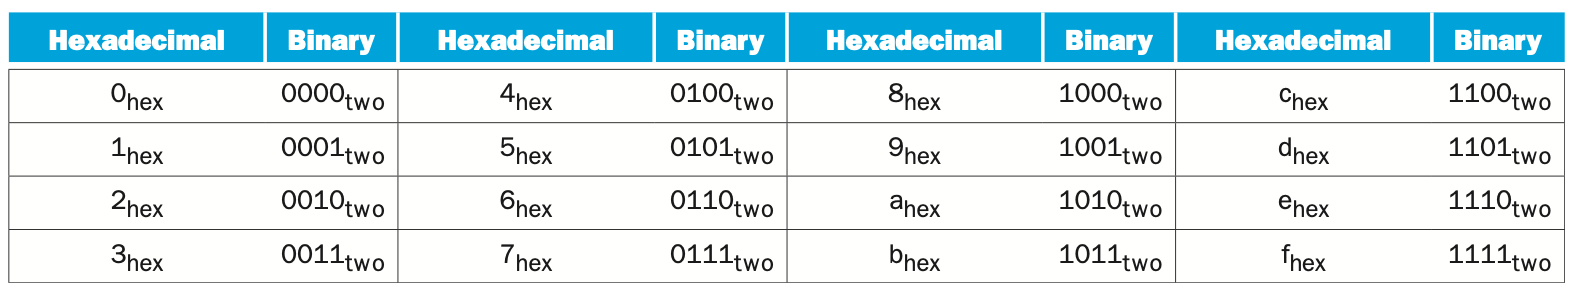
\includegraphics[width=7cm]{8.png}
  \caption{To convert from hexadecimal to binary just replace hexadecimal digit by the corresponding four binary digits and vice versa. If the length of the binary number is not a multiple o 4, go from right to left.}
  \label{fig:}
\end{figure}
\subsubsection{MIPS Fields}
Because computers just read a string of 1's and 0's, how does the computer know where each instruction begins and ends?
When converting from assembly $\longrightarrow$ binary, MIPS instructions are formatted into 32 bits.\\
\textbf{Register Instructions (R-type)}
\begin{figure}[H]
  \centering
 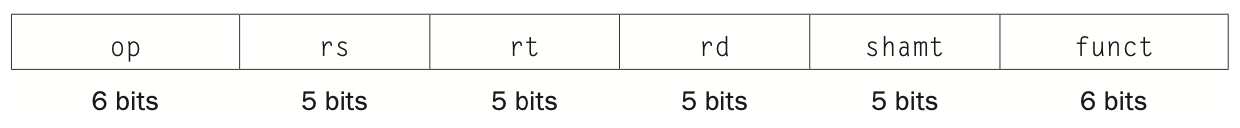
\includegraphics[width=7cm]{9.png}
\caption{The various MIPS fields for R-type (register) instructions.}
  \label{fig:}
\end{figure}

\begin{itemize}
\item op: Basic operation of the instruction, traditionally called the opcode.  The value of this lets computer know meaning of, and size of the following fields.
\item rs: The first register source operand
\item rt: The second register source operand
\item rd: The register destination operand. It gets the result of the operation.
\item shamt: Shift amount. See 2.6 for more details.
\item funct: Function. This field, often called the function code, selects the specific variant of the operation in the op field.
\end{itemize}
\textbf{Immediate Instructions (I-type)}\\

You might have noticed that not all instructions fit into the above format.  For example Let's say you wanted to add a constant to a register and store it in another?  Well, at the moment we would only have $5$-bits available to hold a number, that's not a lot.  The max constant value would be $2^5 - 1 = 31$ (assuming unsigned number), that's not very big.  Instead we have a different instruction format:
\begin{center}
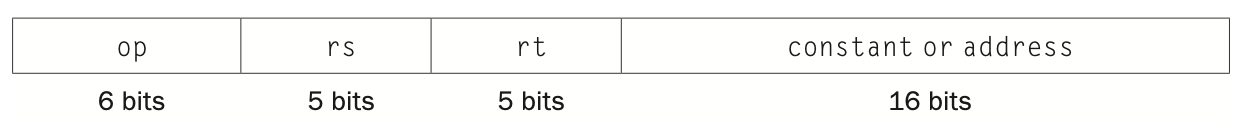
\includegraphics[width=7cm]{10.png}
\end{center}
Note that instructions with this format type are not just add immidiate type instructions, they are also used for load word instructions (among others). The following instruction 
\begin{lstlisting}[style=CStyle, numbers=left, xleftmargin=5.0ex, aboveskip=2em, belowskip=2em, numberstyle=\color{blue}, escapeinside=||]
lw    $t0, 1200($t1)   # $t0 <--- A[300]
add   $t0, $s2, $t0    # $t0 <--- h + A[300]
sw    $t0, 1200($t1)   # A[300] <--- $t0
\end{lstlisting}
is expressed as follows:
\begin{center}
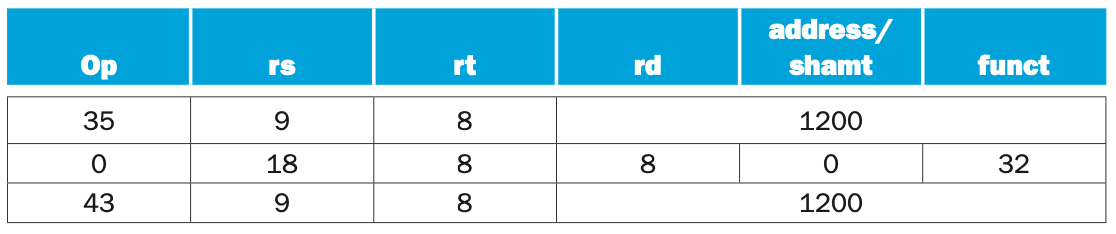
\includegraphics[width=7cm]{11.png}
\end{center}
and in binary:
\begin{center}
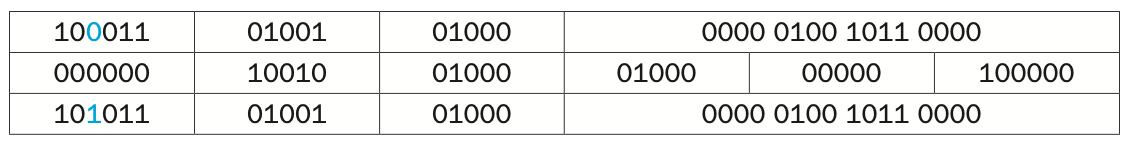
\includegraphics[width=7cm]{12.png}
\end{center}
From this, you can see that each register has an associated reference number:
\begin{center}
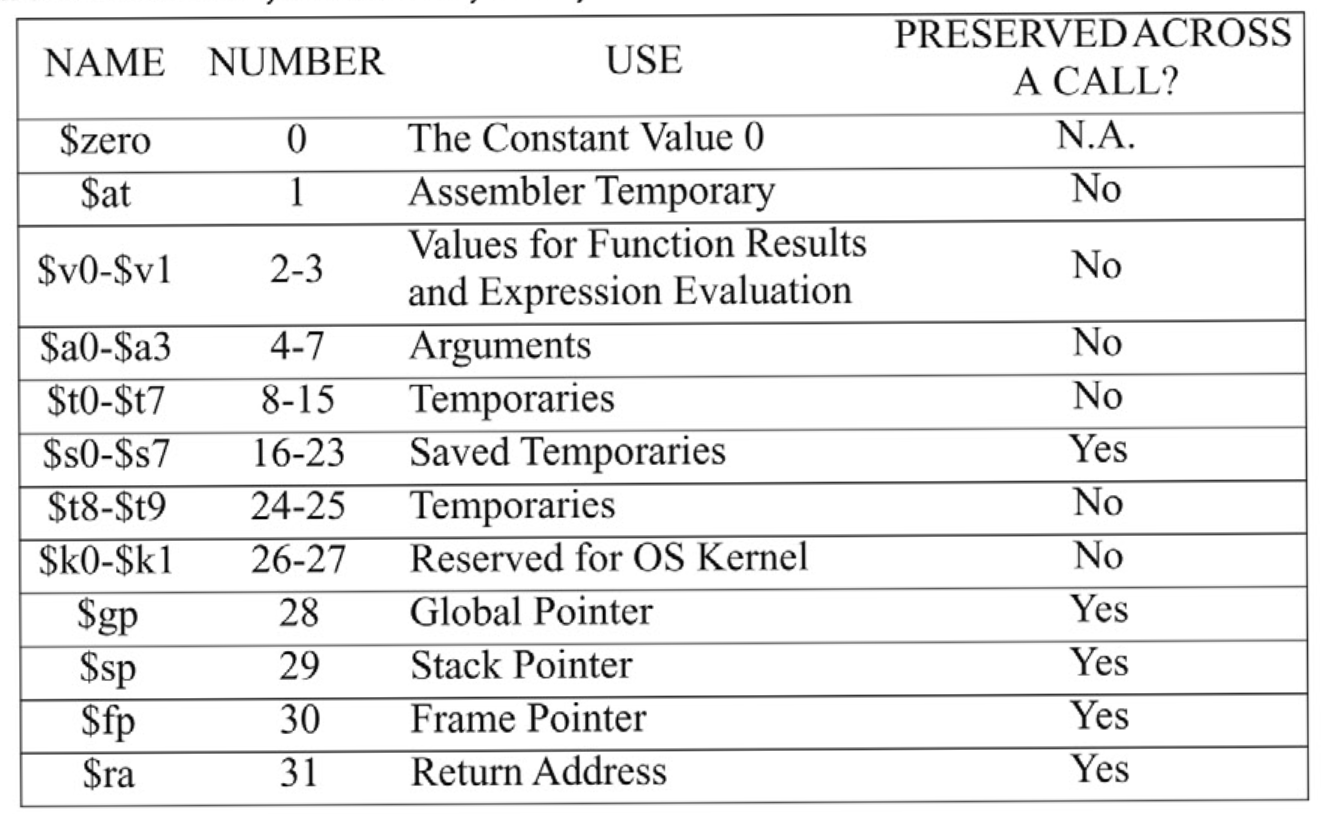
\includegraphics[width=7cm]{13.png}
\end{center}
Here are the opcodes for the instructions we have seen so far:
\begin{center}
  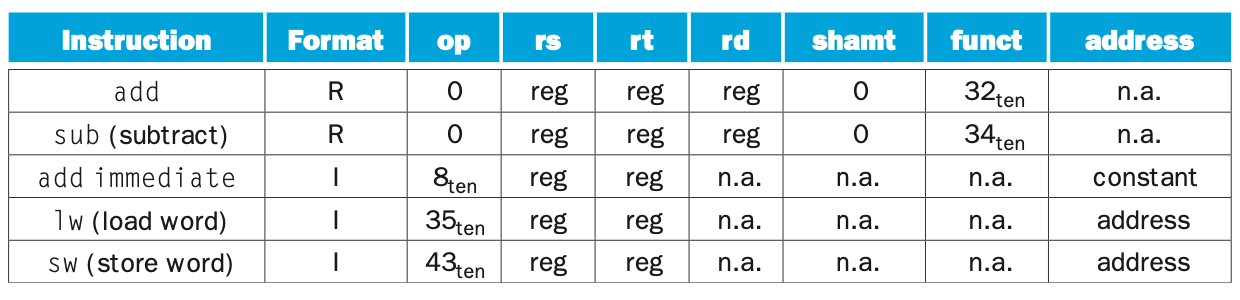
\includegraphics[width=7cm]{14.png}
\end{center}
\subsubsection{Check Yourself}
What MIPS instruction does this represent?
\begin{center}
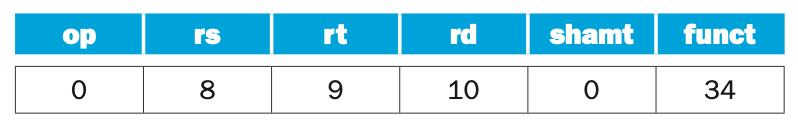
\includegraphics[width=7cm]{15.png}
\end{center}
  \begin{tcolorbox}[%
    enhanced, 
    breakable,
    frame hidden,
    overlay broken = {
      (frame.north west) rectangle (frame.south east);},
    ]
    From the ocode of $0$ and function code of $34$ we know this is a subtract function call.

    We are dealing with registers $8,9,10$ which are \texttt{\$t0}, \texttt{\$t1}, and \texttt{\$t2} respectively.

    Because the MIPS register arguments are orderd \texttt{rd}, \texttt{rs}, \texttt{rt}  we have get the MIPS code
    \begin{lstlisting}[style=CStyle, numbers=left, xleftmargin=5.0ex, aboveskip=2em, belowskip=2em, numberstyle=\color{blue}, escapeinside=||]
sub    $t2, $t0, $t1
\end{lstlisting}

  \end{tcolorbox}
  \addtocounter{subsection}{1}
  \subsection{Instructions for Making Decisions}\label{subsec:}
  \subsubsection{Branch Instructions}
  MIPS has two decision making instructions:
  \begin{itemize}
  \item \texttt{beq register1, register2, L1}\\
    Go to the statement labeled \texttt{L1} if the value in \texttt{register1} equals the value in \texttt{register2};
  \item \texttt{bne register1, register2, L1}\\
    Go to statement labeled \texttt{L1} if value in \texttt{register1} does not equal value in \texttt{register2}. 
  \end{itemize}
  For example, the C code
\begin{lstlisting}[style=CStyle, numbers=left, xleftmargin=5.0ex, aboveskip=2em, belowskip=2em, numberstyle=\color{blue}, escapeinside=||]
if (i == j)
    f = g + h;
else
    f = g-h;
\end{lstlisting}
  where \texttt{f} through \texttt{j} correspond to \texttt{\$s0} through \texttt{\$s4}, corresponds to the MIPS code
\begin{lstlisting}[style=CStyle, numbers=left, xleftmargin=5.0ex, aboveskip=2em, belowskip=2em, numberstyle=\color{blue}, escapeinside=||]
    bne    $s3, $s4, Else
    add    $s0, $s1, $s2     # f = g + h
    j      Exit              # go to Exit

Else:
    sub    $s0, $s1, $s2     # f = g-h

Exit:
\end{lstlisting}
Notice how we did things in reverse; instead of checking for equality (like in the C code), we checked for inequality.
\begin{marginfigure}
The assembler relieves the compiler and the assembly language programmer from the tedium of calculated addresses for branches.
\end{marginfigure}%

\subsubsection{Loops}
How could we use our branch statements to compile the following while Loop:
\begin{lstlisting}[style=CStyle, numbers=left, xleftmargin=5.0ex, aboveskip=2em, belowskip=2em, numberstyle=\color{blue}, escapeinside=||]
while (save[i] == k)
    i += 1;
\end{lstlisting}
where \texttt{i} and \texttt{k} correspond to registers \texttt{\$s3} and \texttt{\$s5}. The address of \texttt{save[0]} is in \texttt{\$s6}.
\begin{lstlisting}[style=CStyle, numbers=left, xleftmargin=5.0ex, aboveskip=2em, belowskip=2em, numberstyle=\color{blue}, escapeinside=||]
Loop:
  sll    $t1, $s3, 2     # $t1 <-- i * 4
  add    $t1, $t1, $s6   # $t1 <-- address of save[i]
  lw     $t0, 0($t1)     # $t0 <-- save[i]
  bne    $t0, $s5, Exit  # if (save[i] != k) Exit
  addi   $s3, $s3, 1     # i += 1
  j      Loop            # go to Loop

Exit:
\end{lstlisting}
\begin{marginfigure}
This is an example of a \textbf{basic block}.  This is a sequence without branches, except possibly at the end, and without branch targets or branch labels, except possibly at the beginning.
\end{marginfigure}%
Because MIPS is byte addressed, to get the memory address of \texttt{save[i]} we need to multiply $i \cdot 4$ and add that to the base address.  We then load that value to a temporary register, and test the condition.

\subsubsection{Unsigned Comparison Tests}
In addition to testing for equality, we might also want to test for less than, or greater than.  To test if less than the instruction ``set on less than''
\begin{lstlisting}[style=CStyle, numbers=left, xleftmargin=5.0ex, aboveskip=2em, belowskip=2em, numberstyle=\color{blue}, escapeinside=||]
  sltu    $t0, $s3, $s4    # $t0 = 1 if $s3 < $s4; otherwise 0
\end{lstlisting}
This sets the destination register to $1$ if less than, and $0$ if not.  An immediate version of this instruction also exists:
\begin{lstlisting}[style=CStyle, numbers=left, xleftmargin=5.0ex, aboveskip=2em, belowskip=2em, numberstyle=\color{blue}, escapeinside=||]
  sltiu    $t0, $s2, 10    # $t0 = 1 if $s2 < 10, 0 otherwise
\end{lstlisting}
\begin{marginfigure}
All relative conditions equal, not equal, less than, less than or equal, greater than, and greater than or equal, can all be created using \texttt{slt}, \texttt{slti}, \texttt{beq}, \texttt{bne}, and \texttt{\$zero} register.   
\end{marginfigure}%
\subsubsection{Signed Comparison Tests}
We have to remember that with negative numbers, the most significant bit is turned on, and so using an unsigned comparison between $-1$ and $5$: $1111_{\text{TWO}} < 0101_{\text{TWO}}$ would return false.  Thus, for signed comparisons we have \texttt{slt} and \texttt{slti}:
\begin{lstlisting}[style=CStyle, numbers=left, xleftmargin=5.0ex, aboveskip=2em, belowskip=2em, numberstyle=\color{blue}, escapeinside=||]
  slt    $t0, $s3, $s4    # $t0 = 1 if $s3 < $s4; otherwise 0
  slti   $t0, $s2, 10    # $t0 = 1 if $s2 < 10, 0 otherwise
\end{lstlisting}

\subsubsection{Bounds Checking Shortcut}
Let's say we want to check if both
\[x < y \quad \text{ and } \quad x \geq 0\]
where $x$ is a and $y$ are signed integers (and $y > 0$).  Assume that \texttt{\$s0} holds $x$ and \texttt{\$s1} holds $y$.   Than we could do
\begin{lstlisting}[style=CStyle, numbers=left, xleftmargin=5.0ex, aboveskip=2em, belowskip=2em, numberstyle=\color{blue}, escapeinside=||]
# Check if x < y
  slt    $t0, $s0, $s1
  beq    $t0, $zero, False

# Check if x >= 0
  slt    $t0, $s0, $zero      # If x < 0
  bne    $t0, $zero, False

# Statement is true
  j      True
\end{lstlisting}
We can actually check for both $x < y$ and $x \geq 0$ in one go by treating $x$ and $y$ as unsigned integers.  The idea here is that since a negative number will have its most significant bit turned on, it looks like a very large unsigned number.  Therefore no matter how large $y$ is, if $x$ is a negative number it will appear as a larger unsigned number.  Thus,
\[0 \leq x \leq y\]
will only be true if $x$ is nonnegative and less than $y$, and when treated as unsigned numbers, testing if $x < y$ will also check if $x \geq 0$:
\begin{lstlisting}[style=CStyle, numbers=left, xleftmargin=5.0ex, aboveskip=2em, belowskip=2em, numberstyle=\color{blue}, escapeinside=||]
sltu $t0, $s0, $s1
beq  $t0, $zero, False
j    True
\end{lstlisting}
This shortcut is really helpful if we want to check if some index is out of bounds for a given array.  For example, let's say we have an array \texttt{example} whose upper bounds $y$.  Then we could use the code above to check if some index $i$ is in bounds ($0 \leq x < y$).

\subsection{Supporting Procedures in Computer Hardware}\label{subsec:}
Thus far, we have only really learned how to perform a sequence of instructions, but what if we want to perform that same sequence of instructions a lot of times, and maybe we want to act upon some variables.  In C we have functions, and in assembly, we have \textbf{procedures}.
\begin{marginfigure}
  A \textbf{procedure} is a stored subroutine that performs a specific task based on the parameters with which it is provided.
\end{marginfigure}%
To perform a procedure in MIPS, we follow the follwoing steps:
  \begin{enumerate}
  \item Put parameters in a place where the procedure can access them.
\item Transfer control to the procedure.
\item Acquire the storage resources needed for the procedure.
\item Perform the desired task.
\item Put the result value in a place where the calling program can access it.
\item Return control to the point of origin, since a procedure can be called from several points in a program.
\end{enumerate}
The following registers are used for procedure calling
\begin{itemize}
\item \texttt{\$a0-\$a3}: four argument registers in which to pass parameters
\item \texttt{\$v0-\$v1}: two value registers in which to return values
\item \texttt{\$ra}: one return address register to return to the point of origin 
\end{itemize}
The return address register is populated by the \textbf{jump-and-link-instruction} (jal):\\

\texttt{jal ProcedureAddress}. 
This instruction simultaneously jumps to ProcedureAddress, and populates the return address register (\texttt{\$ra}) with the address of the following instruction.  This way the computer knows what to perform once the procedure is finished.
\begin{marginfigure}
The \textbf{return address} is a link to the calling site that allows a procedure to return to the proper address; in MIPS it is stored in regeister \texttt{\$ra}. 
\end{marginfigure}%

The \textbf{caller} is the one that puts the parameter values in \texttt{\$a0-\$a3} and uses \texttt{jal X} to jump to procedure \texttt{X} (\textbf{callee}).  Once the callee has finished, it places the results in \texttt{\$v0} and \texttt{\$v1}, and then returns control to the caller using \texttt{jr \$ra}.  This is an unconditional jump to the address specified in a register.

To make all of this work, we need to store the address of the current instruction being executed.  We do this in a register called the \textbf{program counter} (PC). The \texttt{jal} instruction saves PC + 4 in register \texttt{\$ra}.

\subsubsection{Nested Procedures}
Let's say you have the following program:
\begin{lstlisting}[style=CStyle, numbers=left, xleftmargin=5.0ex, aboveskip=2em, belowskip=2em, numberstyle=\color{blue}, escapeinside=||]
#include <stdio.h>

int fact(int n)
{
    if (n < 1)
        return 1;
    else
        return (n * fact(n-1));
}

int main() {
    int result = fact(3);
    printf("%d\n", result);
    return 0;
}
\end{lstlisting}
Because \texttt{fact(n)} can call itself, you have to be careful about saving the return address register (\texttt{\$ra}), as well as any other registers that may be used (more info below).  We can write the above program in MIPS as follows:
\begin{lstlisting}[style=CStyle, numbers=left, xleftmargin=5.0ex, aboveskip=2em, belowskip=2em, numberstyle=\color{blue}, escapeinside=||]
main:
  addi    $a0, $zero, 3
  jal     fact
  add     $a0, $v0, $zero # store result for printing
  addi    $v0, $zero, 1   # print int syscall
  syscall
  addi    $v0, $zero, $10 # exit syscall
  syscall
  
fact:
  addi    $sp, $sp, -8    # make space for two items on stack
  sw      $ra, 4($sp)     # save return address
  sw      $a0, 0($sp)     # save arg n
  slti    $t0, $a0, 1     # test if n < 1
  beq     $t0, $zero, L1  # if n >= 1, goto L1
  lw      $ra, 4($sp)     # restore $ra
  lw      $a0, 0($sp)     # restore arg n
  addi    $v0, $zero, 1   # return 1
  addi    $sp, $sp, 8     # pop two items from stack
  jr      $ra             # return to caller

L1:
  addi    $a0, $a0, -1    # n += -1
  jal     fact            # calls fact and $ra <-- PC+4
  lw      $a0, 0($sp)     # restore arg n
  lw      $ra, 4($sp)     # restore $ra
  addi    $sp, $sp, 8     # Pops two items from stack
  mul     $v0, $a0, $v0   # return n*fact(n-1)
  jr      $ra             # return to caller
\end{lstlisting}
Let's look at how the register values, and stack changes as we go through the program:
\begin{enumerate}
\item In \texttt{main} (before first call of fact):
  \begin{lstlisting}[style=CStyle, xleftmargin=5.0ex, aboveskip=1em, belowskip=1em, escapeinside=..]
$a0 <--- 3
$ra <--- return to main
\end{lstlisting}
  
\item During first call of \texttt{fact(3)}
  \begin{lstlisting}[style=CStyle,  xleftmargin=5.0ex, aboveskip=1em, belowskip=1em, escapeinside=..]
                             Stack
                         --------------
                        |  ra of main  |
                         --------------  <--- -4
                        |      3       |
                         --------------  <--- -8
\end{lstlisting}
\pagebreak
\item First break to \texttt{L1}:
\begin{lstlisting}[style=CStyle, xleftmargin=5.0ex, aboveskip=1em, belowskip=1em, escapeinside=..]
$a0 <-- 3-1 = 2              Stack
$ra <-- return to L1     --------------
                        |  ra of main  |
                         --------------  <--- -4
                        |      3       |
                         --------------  <--- -8
\end{lstlisting}

\item During second call to \texttt{fact(2)}
\begin{lstlisting}[style=CStyle, xleftmargin=5.0ex, aboveskip=2em, belowskip=2em, escapeinside=..]
$a0 = 3-1 = 2                Stack
$ra = return to L1       --------------
                        |  ra of main  |
                         --------------  <--- -4
                        |      3       |
                         --------------  <--- -8
                        |   ra of L1   |
                         --------------  <--- -12
                        |      2       |
                         --------------  <--- -16
\end{lstlisting}

\item During second break to \texttt{L1}
\begin{lstlisting}[style=CStyle, xleftmargin=5.0ex, aboveskip=1em, belowskip=1em, escapeinside=..]
$a0 <--- 2-1 = 1             Stack
$ra <--- return to L1    --------------
                        |  ra of main  |
                         --------------  <--- -4
                        |      3       |
                         --------------  <--- -8
                        |   ra of L1   |
                         --------------  <--- -12
                        |      2       |
                         --------------  <--- -16
\end{lstlisting}

\item During third call to \texttt{fact(1)}
\begin{lstlisting}[style=CStyle, xleftmargin=5.0ex, aboveskip=1em, belowskip=1em, escapeinside=..]
$a0 = 1                Stack
$ra = return to L1       --------------
                        |  ra of main  |
                         --------------  <--- -4
                        |      3       |
                         --------------  <--- -8
                        |   ra of L1   |
                         --------------  <--- -12
                        |      2       |
                         --------------  <--- -16
                        |   ra of L1   |
                         --------------  <--- -20
                        |      1       |
                         --------------  <--- -24
\end{lstlisting}

\item During third break to \texttt{L1}
\begin{lstlisting}[style=CStyle, xleftmargin=5.0ex, aboveskip=1em, belowskip=1em, escapeinside=..]
$a0 <--- 1-1 = 0             Stack
$ra <--- L1              --------------
                        |  ra of main  |
                         --------------  <--- -4
                        |      3       |
                         --------------  <--- -8
                        |   ra of L1   |
                         --------------  <--- -12
                        |      2       |
                         --------------  <--- -16
                        |   ra of L1   |
                         --------------  <--- -20
                        |      1       |
                         --------------  <--- -24
\end{lstlisting}

\item During fourth call to \texttt{fact(0)} 
\begin{lstlisting}[style=CStyle, xleftmargin=5.0ex, aboveskip=1em, belowskip=1em, escapeinside=..]
$a0 = 0                      Stack
$ra = L1                 --------------
                        |  ra of main  |
$ra <-- stack[-28] = L1  --------------  <--- -4
$a0 <-- stack[-32] = 0  |      3       |
$v0 <-- 1 * 1 = 1        --------------  <--- -8
                        |   ra of L1   |
                         --------------  <--- -12
                        |      2       |
                         --------------  <--- -16
                        |   ra of L1   |
                         --------------  <--- -20
                        |      1       |
                         --------------  <--- -24
                        |   ra of L1   |
                         --------------  <--- -28
                        |      0       |
                         --------------  <--- -32$
\end{lstlisting}
\pagebreak
\item Backtracking to 3rd \texttt{L1}: 
\begin{lstlisting}[style=CStyle, xleftmargin=5.0ex, aboveskip=1em, belowskip=1em, escapeinside=..]
$ra <-- stack[-20] = L1      Stack
$a0 <-- stack[-24] = 1   --------------
$v0 <-- 1 * 1 = 1       |  ra of main  |
                         --------------  <--- -4
                        |      3       |
                         --------------  <--- -8
                        |   ra of L1   |
                         --------------  <--- -12
                        |      2       |
                         --------------  <--- -16
                        |   ra of L1   |
                         --------------  <--- -20
                        |      1       |
                         --------------  <--- -24$
\end{lstlisting}

  \item Backtracking to 2nd \texttt{L1}: 
\begin{lstlisting}[style=CStyle, xleftmargin=5.0ex, aboveskip=1em, belowskip=1em, escapeinside=..]
$ra <-- stack[-12] = L1      Stack
$a0 <-- stack[-16] = 2   --------------
$v0 <-- 1 * 2 = 2       |  ra of main  |
                         --------------  <--- -4
                        |      3       |
                         --------------  <--- -8
                        |   ra of L1   |
                         --------------  <--- -12
                        |      2       |
                         --------------  <--- -16$
\end{lstlisting}

  \item Backtracking to 1st \texttt{L1}: 
\begin{lstlisting}[style=CStyle, xleftmargin=5.0ex, aboveskip=1em, belowskip=1em, escapeinside=..]
$ra <-- stack[-4] = main     Stack
$a0 <-- stack[-8] = 3    --------------
$v0 <-- 2 * 3 = 6       |  ra of main  |
                         --------------  <--- -4
                        |      3       |
                         --------------  <--- -8$
\end{lstlisting}

  \item Back in main
\begin{lstlisting}[style=CStyle, xleftmargin=5.0ex, aboveskip=1em, belowskip=1em, escapeinside=||]
$a0 <-- 6
$v0 <-- 1
Print 1
Exit
\end{lstlisting}
\end{enumerate}
If you examine things closely, you can actually forgoe the restoring of \texttt{\$ra} and \texttt{\$a0} inside of fact, since those remain unchanged.
\begin{marginfigure}
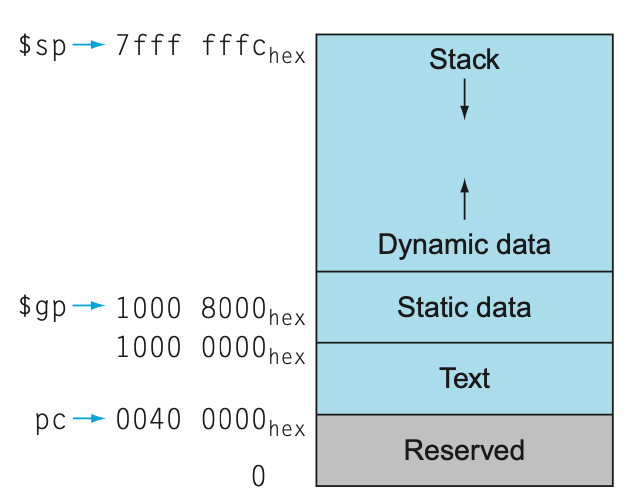
\includegraphics[width=\linewidth]{16.png}
  \caption{How the memory is split up.}
\end{marginfigure}%

\subsubsection{Calling Conventions}

\textbf{Rules for all calls}
\begin{itemize}
\item The first instruction in the function manipulates \texttt{\$sp} to allocate $F$ words of stack:
  \[\texttt{addi \$sp, \$sp, -F*4}\]
  where $F = A + L + P + (1 \text{ for } \texttt{\$ra} \text{ if needed }) + (1 \text{ for } \texttt{\$fp} \text{ if in use }) + (2 \text{ for } \texttt{\$gp}) + \text{ padding }$. Also, $F$ is the frame size in words, and should be even.\\
  Corollary 1: \texttt{\$sp} is not changed at any other point than the first and last instructions in the function.
\begin{marginfigure}
  \begin{center}
    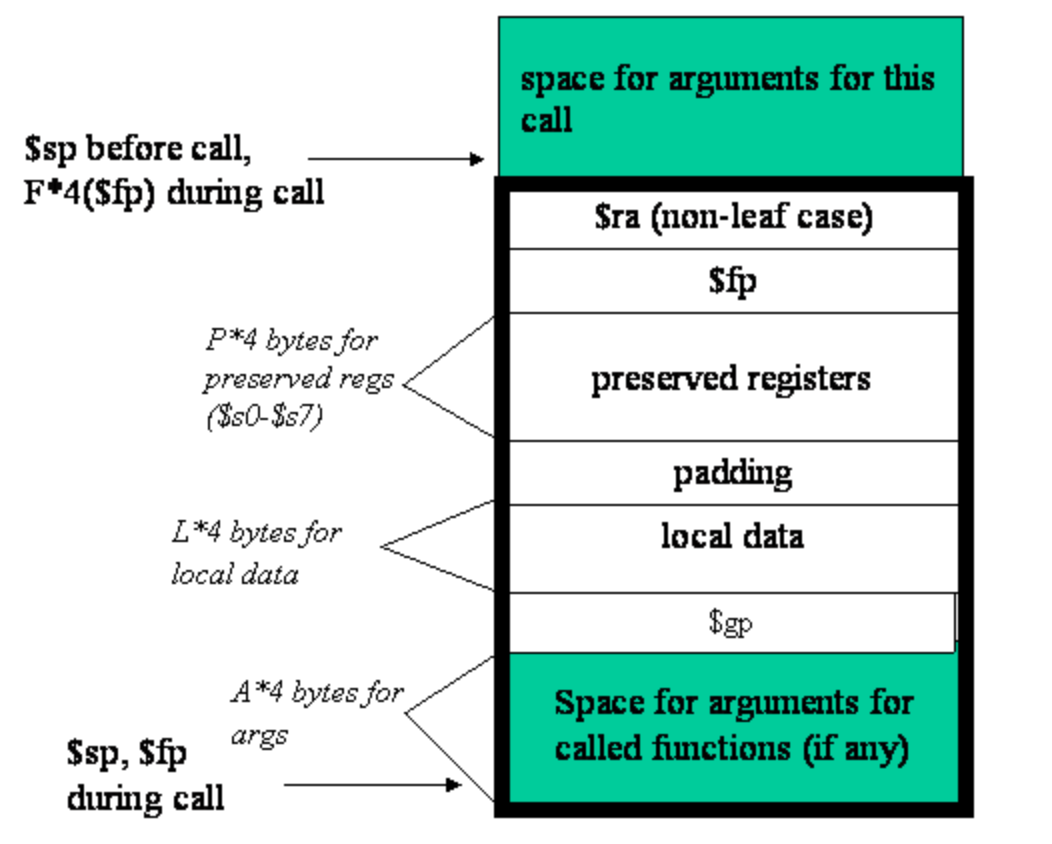
\includegraphics[width=\linewidth]{17.png}
  \end{center}
  \caption{Stack organization during call}
\end{marginfigure}%
\item If you want to use any preserved register in any place during the function, you must store them into the stack when you \textbf{enter} the function (not when you use it). Let's assume we are saving \texttt{\$s0}, \texttt{\$s1}, and \texttt{\$s2} registers, as well as \texttt{\$ra} and \texttt{\$sp}. Then we would write:
\begin{lstlisting}[style=CStyle, numbers=none, xleftmargin=5.0ex, aboveskip=1em, belowskip=1em, numberstyle=\color{blue}, escapeinside=||]
sw $ra, (F-1)*4($sp)   # Not needed for leaf functions
sw $fp, (F-2)*4($sp)
sw $s2, (F-3)*4($sp)
sw $s1, (F-4)*4($sp)
sw $s0, (F-5)*4($sp)
\end{lstlisting}
\item After saving preserved registers, copy \texttt{\$sp} into \texttt{\$fp}, so that from now until you start returning, you can use offsets from \texttt{\$fp} to access the locations.  Save and restore local variables as needed after this point, using \texttt{\$fp} and the spots already allocated for them on the stack.
\item You may pass information \textbf{into} a function only through \texttt{\$a0-\$a3} and extra stack arguments.  As the called function, you may not use the value held in any other register except \texttt{\$sp}, \texttt{\$fp}, \texttt{\$gp} and \texttt{\$ra} (i.e. don't try and use \texttt{\$v0} or \texttt{\$s0}).  The $#4$ (fifth) argument to the current function is available at $(F+4)*4(\texttt{\$fp})$.  You may store argument $0$ from \texttt{\$a0} into its reserved spot at $F*4(\$fp)$, arg1 into $(F+1)*4(\texttt{\$fp})$, etc., if you want.

\item You may pass information \textbf{out of} a function through only \texttt{\$v0-\$v1}.
\item You may only enter a function at its beginning.  You may not \texttt{jal} into the middle of a function.
\item You may have only one \texttt{jr \$ra} in each function. It is the last instruction in the function, following the instructions that restore the registers saved.   
\end{itemize}

\textbf{Extra rules for non-leaf functions}:
\begin{itemize}
\item Look at the declarations for all procedures this function \textit{might} call. Find the one with the largest number of arguments, $A$, and then make $A$ at least $4$.  You must allocate $A \cdot 4$ bytes on the stack upon entry into your function.
\item If passing more than $4$ arguments, then place $4$ arguments into \texttt{\$a0-\$a3}.  Every argument past the $4^{\text{th}}$ argument is placed on the stack.  For example suppose $6$ arguments are in \texttt{\$s0-\$s5}:
\begin{lstlisting}[style=CStyle, numbers=none, xleftmargin=5.0ex, aboveskip=2em, belowskip=2em, numberstyle=\color{blue}, escapeinside=||]
move $a0, $s0    # 0($fp) reserved on the stack
move $a1, $s1    # 4($fp) reserved on the stack
move $a2, $s2    # 8($fp) reserved on the stack
move $a3, $s3    # 12($fp) reserved on the stack
sw $s4, 16($fp)  # 5th arg in the stack. Always here!
sw $s5, 20($fp)  # 5th arg in the stack. Always here!
\end{lstlisting}
\item You must preserve register \texttt{\$ra} because a called-function \texttt{jal} destroys the value, and it is a preserved register. 
\end{itemize}
\addtocounter{subsection}{1}
\subsection{MIPS Addressing for 32-bit Immediates and Addresses}\label{subsec:}
\subsubsection{32-bit Constant into Register}
If you have been following closely, you may have noticed that when adding a constant to a register there are only $16$ bits available for the constant (as it is an I-type instruction):
\begin{lstlisting}[style=CStyle, numbers=none, xleftmargin=5.0ex, aboveskip=1em, belowskip=1em, numberstyle=\color{blue}, escapeinside=..]
 ------ ----- ----- ----------------
|  op  |  rt |  rs |    constant    |
 ------ ----- ----- ----------------
   6      5     5          16
\end{lstlisting}
The question then remains, what do you do if you want to place a constant larger than $16$ bits?  You achieve this with the following two instructions:
\begin{enumerate}
\item \texttt{lui rt, immediate}\\
  which loads immediate value into the upper $16$ bits of \texttt{rt} and zeros lower $16$ bits.
\item \texttt{ori rt, rs, immediate}\\
  Bitwise or of \texttt{rs} and \texttt{immediate} placed into \texttt{rt} (\texttt{rt <-- rs | imm}).  
\end{enumerate}
\begin{marginfigure}
A word of caution.  Using the instruction \texttt{addi} sign extends the msb of immediate. 
\end{marginfigure}%
\subsubsection{Branch Addressing}
Branch instructions take are I-type instructions:
\begin{lstlisting}[style=CStyle, numbers=none, xleftmargin=5.0ex, aboveskip=1em, belowskip=1em, numberstyle=\color{blue}, escapeinside=..]
 ------ ----- ----- ----------------
|  op  |  rs |  rt |encoded address |
 ------ ----- ----- ----------------
   6      5     5         16
\end{lstlisting}
The target of the encoded addres is
\[\text{Target} = 4(\text{encoded address}) + \texttt{PC} + 4.\]
That is, branch instructions are word addressed ($4(\text{encoded address})$), and relative to the next instruction ($\texttt{PC} + 4$).

\subsubsection{Jump Addressing}
Jump instructions are J-type instructions:
\begin{lstlisting}[style=CStyle, numbers=none, xleftmargin=5.0ex, aboveskip=1em, belowskip=1em, numberstyle=\color{blue}, escapeinside=..]
 ------ --------------------------
|  op  |      encoded address     |
 ------ --------------------------
   6               26
\end{lstlisting}
In this case the lower $28$ bits of the address to be jumped to are
\[4 \cdot \text{encoded address}\]
and the upper four are that of the \texttt{PC}.  If you need to jump to a really far away address (more than 64 million instructions away), then you use jump register instruction (\texttt{jr}).
\addtocounter{subsection}{1}
\subsection{Translating and Starting a Program}\label{subsec:}
\begin{figure}[H]
  \centering
  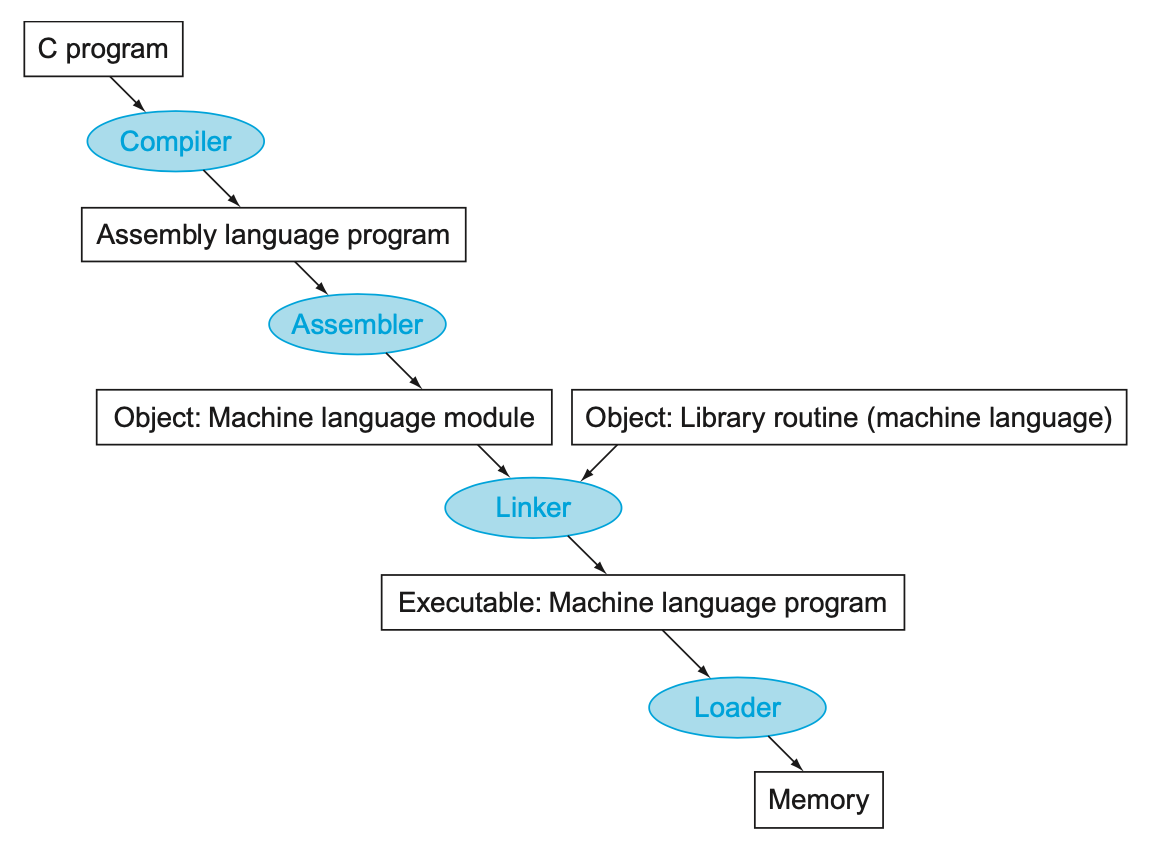
\includegraphics[width=8cm]{18.png}
  \caption{The four steps that go into loading your C program into memory.}
  \label{fig:}
\end{figure}
\subsubsection{Compiler}
The compiler transforms the C program into an assembly language program.

\subsubsection{Assembler}
The main job of the assembler is to convert assembly language into binary machine code (object file). The assembler must determine the addresses associated with labels, which it keeps track of in a symbol table which contains pairs of symbols and addresses.  The object for UNIX systems typically contains six distinct pieces:
\begin{itemize}
\item The \textit{object file header} describes the size and position of the other pieces of the object file.
\item The \textit{text segment} contains the machine language code.
\item The \textit{static data segment} contains data allocated for the life of the program. (UNIX allows programs to use both static data, which is allocated throughout the program, and dynamic data, which can grow or shrink as needed by the program.)
\item \textit{The relocation information} identifies instructions and data words that depend on absolute addresses when the program is loaded into memory.
\item The \textit{symbol table} contains the remaining labels that are not defined, such as external references.
\item The \textit{debugging information} contains concise descriptions of how the modules were compiled so that a debugger can associate machine instructions with C source files and make data structures readable.
\end{itemize}
\subsubsection{Linker}
The linker or link editor is a systems program that combines independently assembled machine language programs and resolves all undefined labels into an executable file.  In this way, you can combine your program with other progras (such as header files or libraries) without having to recompile everything together.
\subsubsection{Loader}
The loader places an object program in main memory so that it is ready to execute.  The loader follows the following steps in UNIX systems:
\begin{enumerate}
\item Reads the executable file header to determine size of the text and data segments.
\item Creates an address space large enough for the text and data.
\item Copies the instructions and data from the executable file into memory.
\item Copies the parameters (if any) to the main program onto the stack.
\item Initializes the machine registers and sets the stack pointer to the first free location.
\item Jumps to a start-up routine that copies the parameters into the argument registers and calls the main routine of the program. When the main routine returns, the start-up routine terminates the program with an \texttt{exit} system call.
\end{enumerate}

\addtocounter{subsection}{1}
\subsection{Arrays versus Pointers}\label{subsec:}
Let's look at two ways we can set an array to all zeros: one using pointers, and one using arrays, so that we get an idea for how C pointers work.

\subsubsection{Array}
Let's say that we have the following C code:
\begin{lstlisting}[style=CStyle, numbers=left, xleftmargin=5.0ex, aboveskip=2em, belowskip=2em, numberstyle=\color{blue}, escapeinside=||]
clear1(int array[], int size)
{
    int i;
    for (i = 0; i < size; i +=1)
        array[i] = 0;
}
\end{lstlisting}
Then we would have the following MIPS code:
\begin{lstlisting}[style=CStyle, numbers=left, xleftmargin=5.0ex, aboveskip=2em, belowskip=2em, numberstyle=\color{blue}, escapeinside=..]
  addiu  $sp, $sp, $-16       # Space for four arguments
  addi   $sp, $sp, $-32       # Space for array of 8 words
  addi   $sp, $sp, $-4        # Space for $gp
  addi   $sp  $sp, $-4        # space for $fp
  addi   $sp  $sp  $-4        # Space for $ra

F = 4(arguments) + 8(local data) + 1(ra) + 1(fp) + 2(gp)
  = 16
Stack
 ------------
|     ra     |
 ------------ <--- +60
|     fp     |
 ------------ <--- +56
|  array[7]  |
 ------------ <--- +52
|  array[6]  |
 ------------ <--- +48
|  array[5]  |
 ------------ <--- +44
|  array[4]  |
 ------------ <--- +40
|  array[3]  |
 ------------ <--- +36
|  array[2]  |
 ------------ <--- +32
|  array[1]  |
 ------------ <--- +28
|  array[0]  |
 ------------ <--- +24
|            |
 ------------ <--- +20
|     gp     |
 ------------ <--- +16
| arg 3 spce |
 ------------ <--- +12
| arg 2 spce |
 ------------ <--- +8
| arg 1 spce |
 ------------ <--- +4
| arg 0 spce |
 ------------ <--- +0

main:
  addiu  $sp, $sp, -64        # Allocate stack space
  sw     $ra, 60($sp)         # Save return address
  sw     $fp, 56($sp)         # Save frame pointer
  sw     $gp, 16($sp)         # Save global pointer
  add    $fp, $sp, $zero      # Estabilish frame pointer
  addiu  $a0, $fp, 24         # arg0 <--- &array[0]
  addiu  $a1, $zero, 8        # arg1 <--- size = 8
  jal    clear1               # clear1(&array, 8)
  ...
  j      exit

clear1:
  add    $t0, $zero, $zero    # i <-- 0
  slti   $t3, $a1,   1        # $t3 <-- 1 if size < 1
  bne    $t3, $zero, exit     # if (size < 1) exit

loop:
  sll    $t1, $t0, 2          # $t1 <-- i * 4
  add    $t2, $a0, $t1        # $t2 <-- mem address of array[i]
  sw     $zero, 0($t2)        # array[i] <-- 0
  addi   $t0, $t0, 1          # i += 1
  slt    $t3, $t0, $a1        # $t3 <-- i, if i < size
  bne    $t3, $zero, Loop     # goto loop if i

exit:
\end{lstlisting}
\begin{marginfigure}
Note that this code only works if \texttt{size > 0}; ANSI C requires a test of size before the loop, but we'll skip that legality here.  
\end{marginfigure}%
\section{Arithmetic for Computers}
\addtocounter{subsection}{1}
\subsection{Addition and Subtraction}\label{subsec:}
Addition in binary works just like addition in decimal, going bit by bit, and carrying over:
\begin{lstlisting}[style=CStyle, numbers=none, xleftmargin=5.0ex, aboveskip=0.5em, belowskip=0.5em, numberstyle=\color{blue}, escapeinside=||]
  10_{10} = 01010_2
+  6_{10} = 00110_2
  ----------------
  16_{10} = 10000_{2}
\end{lstlisting}
Subtraction can either be done via the subtract operation, or by adding a negative number (in two's complement):
\begin{center}
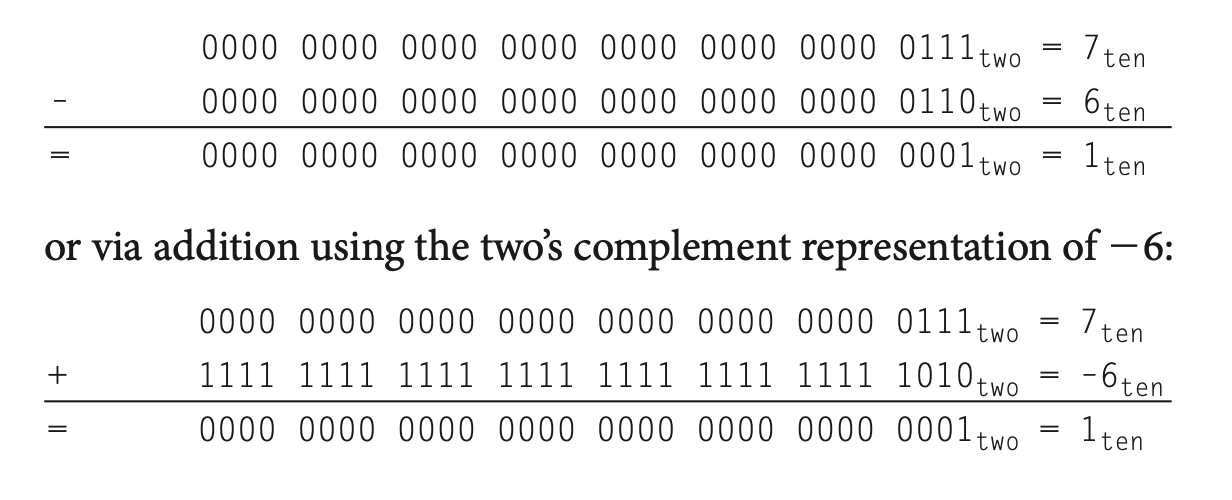
\includegraphics[width=9cm]{19.png}
\end{center}
\subsubsection{Overflow Twos Complement}
\textbf{Addition}
\begin{itemize}
\item Cannot occur when adding operands with different signs. This is because the sum can be no larger than one of the numbers, and both numbers fit.
\item Overflow can be detected when adding numbers of the same sign but the sign bit changes.
\end{itemize}
\textbf{Subtraction}
\begin{itemize}
\item Cannot occur when signs are the same $(a - b = a + (-b))$.
\item Overflow occurs when we subtract a negative number from a positive number but get a negative number $(a- (-b) = -x)$
\end{itemize}

\subsubsection{Unsigned Overflow}
Depending upon the situtation, one may or may not want an exception to be thrown when overflow occurs.  For this reason there are there are two types of integer opporations.
\begin{itemize}
\item \texttt{add}, \texttt{addi}, and \texttt{sub} cause exceptions on overflow.
\item \texttt{addu}, \texttt{addiu}, and \texttt{subu} do not cause exceptions on overflow.  
\end{itemize}
Note that C ignores overflows, and so MIPS compilers will always generate the unsigned versions.
\begin{marginfigure}
Note that allthough \texttt{addiu} is unsigned addition, the $16$-bit immediate field is sign extended to $32$-bits and so the immediate field is signed, even if the operation is ``unsigned''. 
\end{marginfigure}%
  \begin{center}
    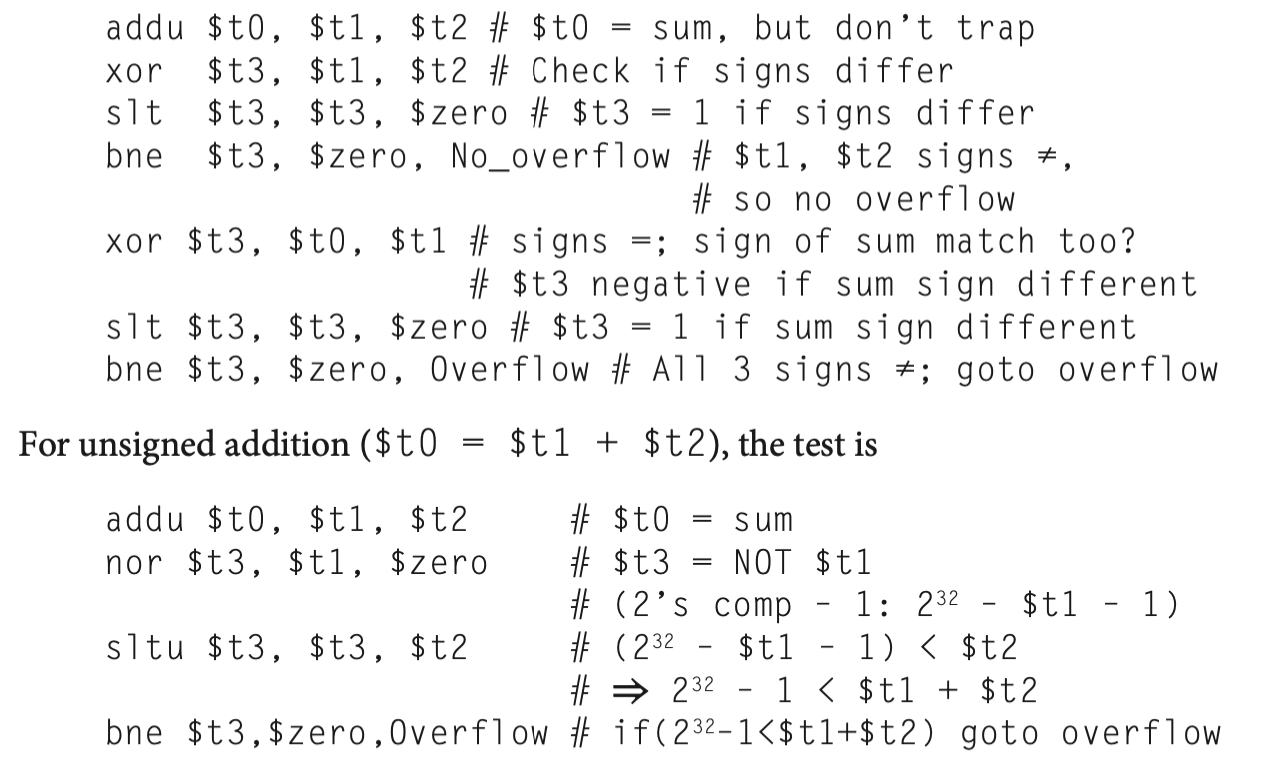
\includegraphics[width=10cm]{20.png}
  \end{center}
  \caption{Because MIPS does not have a conditional branch to test overflow, a sequence of MIPS instructions can discover overflow.}


\subsection{Multiplication}\label{subsec:}
Let's say we want to multiply $1011 \times 0101$, then we would perform the following steps:
\begin{center}
\begin{arithmetic}
           1011 &   \textit{\textcolor{blue}{Multiplicand}}    \\
    \times 0101 &   \textit{\textcolor{blue}{Multiplier}}   \\
           1011 &   \\
          0000~ &   \\
         1011~~ \\
  +     0000~~~ \\
       00110111 & \textit{\textcolor{blue}{Product}}
\end{arithmetic}
\end{center}
Notice that we just add copies of the multiplicand (shifted over by 1 each time), or zero (depending upon bit of multiplier).  Thus, to perform multiplaction, we will need the following pieces of hardware:
\begin{itemize}
\item A multiplicand register. Because we are shifting over the multiplicand each time, it needs to be twice as big (so $64$-bits).
\item A multiplier register. Size of $32$-bits.
\item A product register.  Needs to be $64$ bits wide.
\item An Arithmetic Logic Unit (ALU) to perform the addition of product and multiplicand registers.
\item A control test that in each cycle tells:
  \begin{itemize}
\item the ALU to sum the multiplicand and product (if control says to)
\item the multiplicand to shift left,
\item the multiplier to shift right, 
\item the product register to change or not depending upon the lsb if the multiplier register.
\end{itemize}
\end{itemize}
\begin{figure}[H]
  \centering
  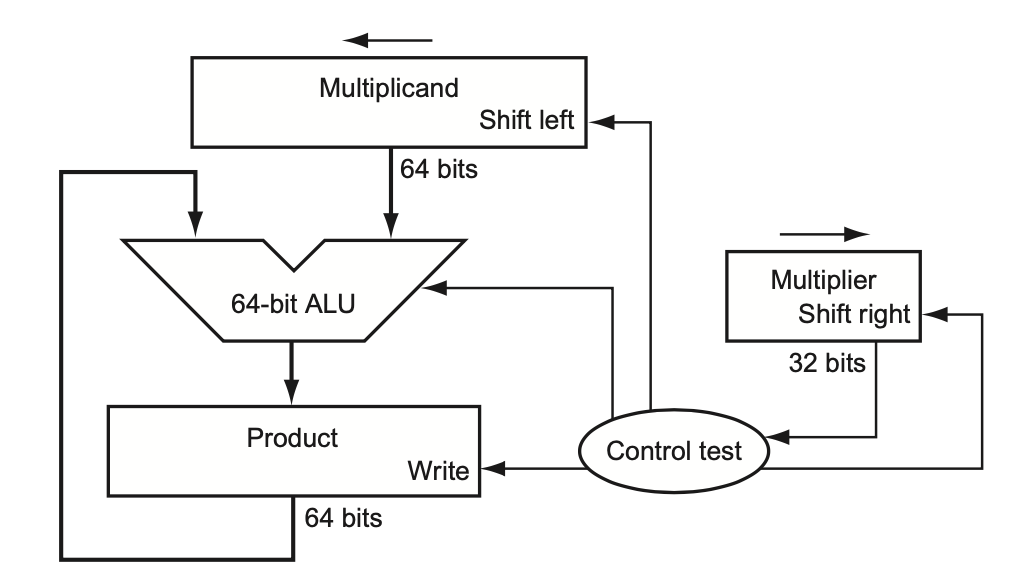
\includegraphics[width=9cm]{21.png}
  \caption{A simple version of multiplication hardware.}
  \label{fig:}
\end{figure}
So what will the first cycle of hardware look like?
\begin{figure}[H]
  \centering
  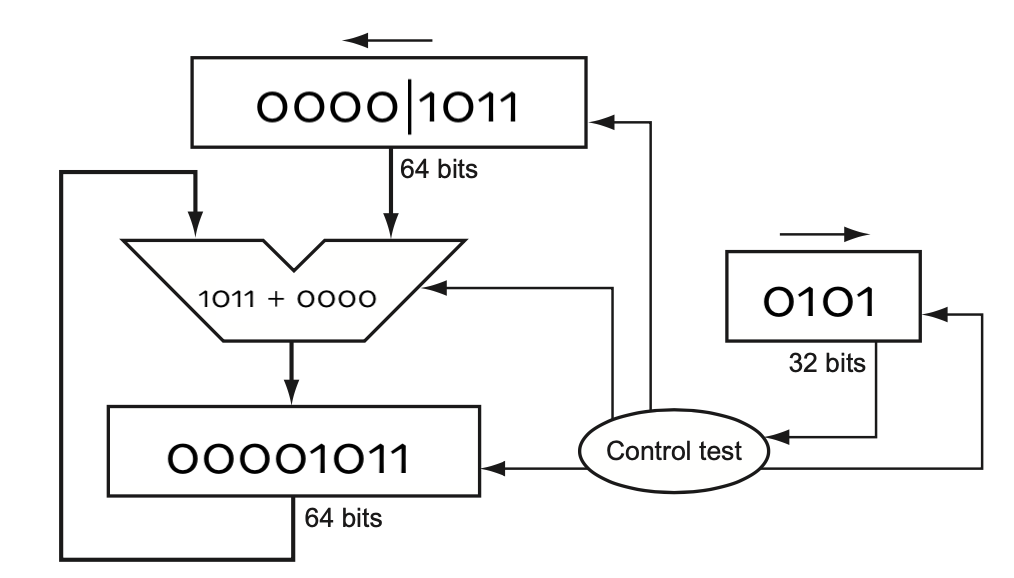
\includegraphics[width=9cm]{23.png}
  \caption{So at first, the product register is set to $0000$, the multiplicand register is set to $1011$, and the multiplier register is set to $0101$. The control test tests the first bit of the multiplicand (1), and so tells the ALU to sum the product and multiplicand registers, and store the value in the product register.  The control then shifts the multiplicand 1 bit to the left, and the multiplier 1 bit to the right.}
  \label{fig:}
\end{figure}
\begin{marginfigure}
  \begin{center}
    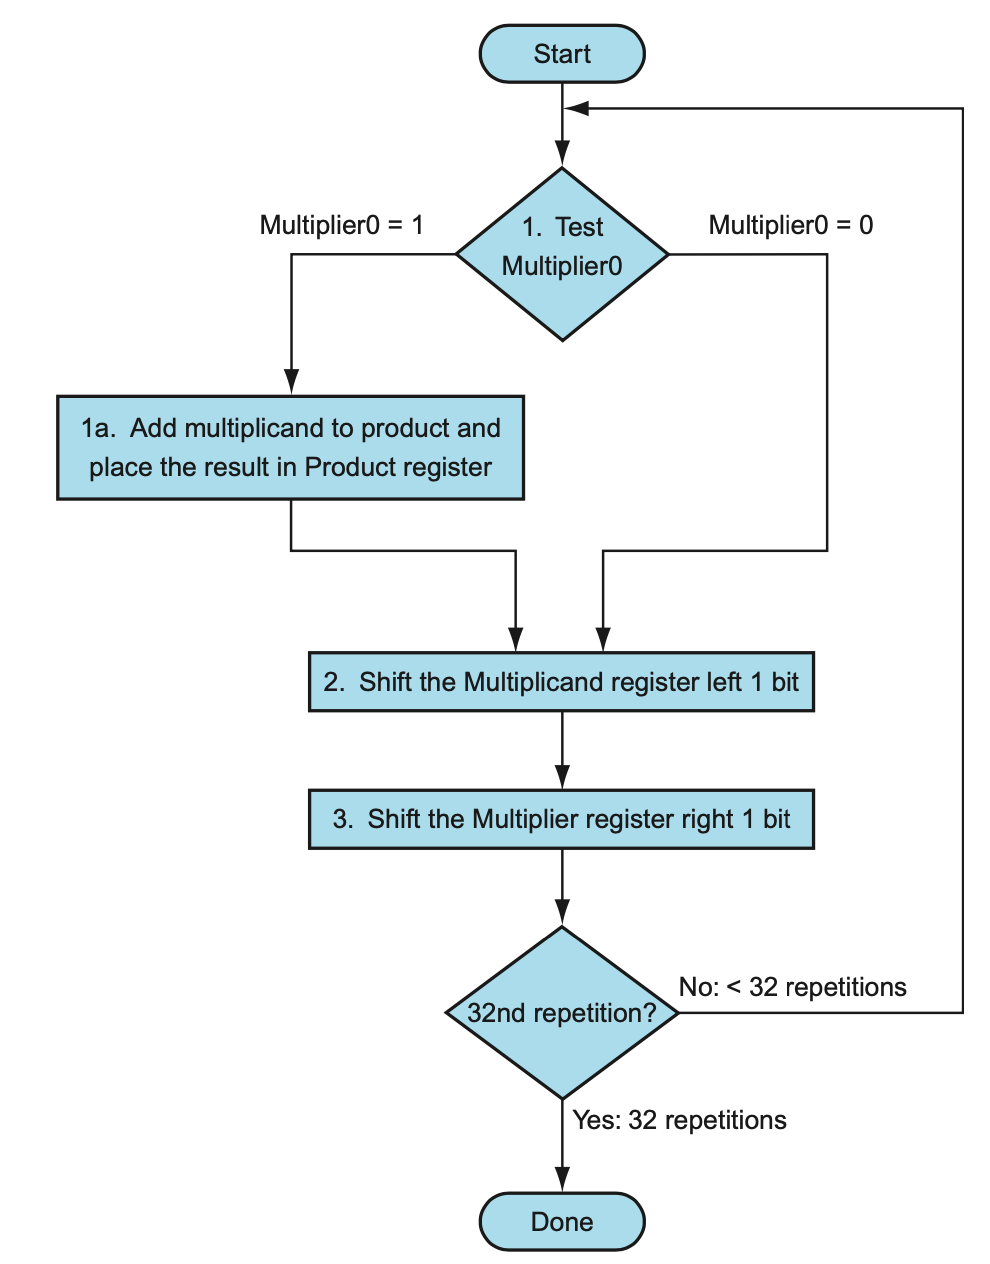
\includegraphics[width=\linewidth]{22.png}
  \end{center}
  \caption{The multiplication algorithm.}
\end{marginfigure}%

\subsubsection{Faster Multiplication}
\textbf{Parallel Processing Speedup}
\begin{itemize}
\item The multiplier and multiplicand are shifted while the multicland is added to the product if the multiplier bit is a 1.
\item The hardware just has to ensure that it tests the right bit of the multiplier and gets the preshifted version of the multiplicand.
\end{itemize}
\textbf{Resource Optimization Speedup}
If you look back at doing the multiplication by hand, you may notice that at each step you are really only adding four bits at once.  What we will do now, is have a 32-bit multiplicand register, a 32-bit adder, and a 64-bit product, and shift the product register instead of the multiplicand register.  Let's se how this works in practice.
\begin{itemize}
\item \textbf{Step 1}\\
  \begin{aligned}
    \text{Multiplicand: }&1011\\
    \text{Multiplier: }&0101\\
    \text{Product: }&1011 \; 0000 
  \end{aligned}

  \item \textbf{Step 2}\\
  \begin{aligned}
    \text{Multiplicand: }&1011\\
    \text{Multiplier: }&0101\\
    \text{Product: }&0101 \; 1000 
  \end{aligned}

  \item \textbf{Step 3}\\
  \begin{aligned}
    \text{Multiplicand: }&1011\\
    \text{Multiplier: }&0101\\
    \text{Product: }&1101 \; 1100
  \end{aligned}
  \item \textbf{Step 4}\\
  \begin{aligned}
    \text{Multiplicand: }&1011\\
    \text{Multiplier: }&0101\\
    \text{Product: }&0110 \; 1 110
  \end{aligned}\\
The last shift will then set the product as $0011 \; 0111$.
\end{itemize}
\begin{marginfigure}
  \begin{center}
    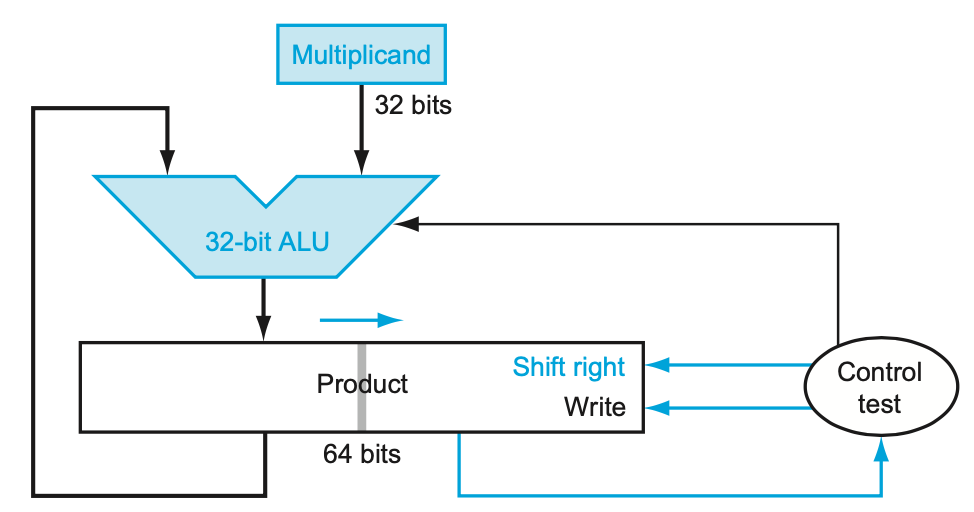
\includegraphics[width=\linewidth]{24.png}
  \end{center}
  \caption{The faster multiplication hardware, taking advantage of parallel processing as well as reduced register size}
\end{marginfigure}%

\subsubsection{Even Faster Multiplication}

\subsection{Division}\label{subsec:}
Let's first examine a little bit more closely the long division from elementary school:
\[\intlongdivision{1001010}{1000}.\]
Notice how as we are testing to see the divisor is less than the $n$ MSBs of the dividend  where $n$ increases by 1 each cycle.  If the divisor is less than, we subtract the divisor from the dividend and put 1 in the quotient.

So how does all of this transfer over to hardware?
\begin{itemize}
\item Well, so that we are comparing divisor to the MSBs of the divident we will store the 32-bit divisor in a 64-bit integer, but start with it in the 32 MSBs.  This way, after each cycle we just shift the divisor to the right one.
\item Because we keep subtracting from the dividend, we just make our life simple and start the dividend as the remainder.
\item Instead of placing the $1$ or $0$ of the quotient starting from the LSB, we place start with the quotient as zero and shift the quotient left $1$ and set LSB to 1 if applicable.  This way at the end this will get shifted over to become the MSB.
\end{itemize}
\begin{marginfigure}
  \begin{center}
    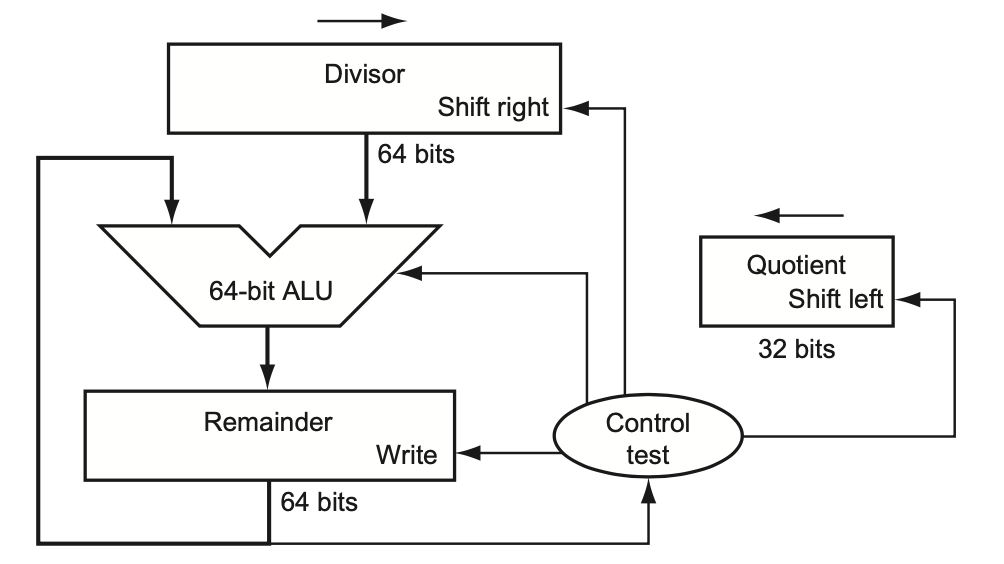
\includegraphics[width=\linewidth]{37.png}
  \end{center}
  \caption{Hardware implementation of division}
\end{marginfigure}%
\begin{figure}[H]
  \centering
  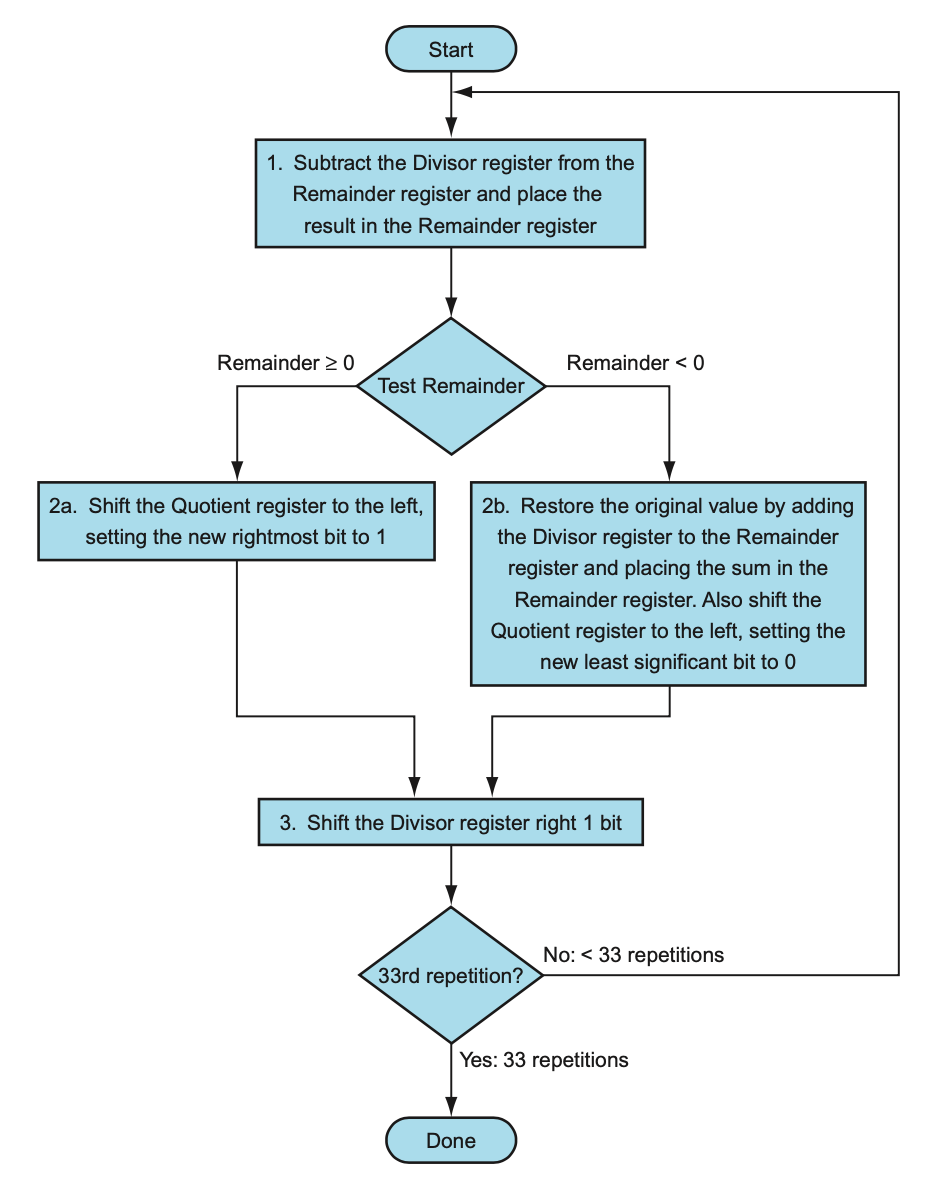
\includegraphics[width=7cm]{36.png}
  \caption{The division algorithm that we will implement in hardware.}
  \label{fig:}
\end{figure}

\subsubsection{Faster Division}
We can make this a little bit more efficient. Instead of shifting the divisor right, we can shift the remainder/quotient left.  So we start with the quotient in the 32 LSBs, shift the remainder left one cycle and compare the 32 MSBs of the remainder with the divisor (we want the divisor to be less than the upper 32 MSBs of the quotient/remainder).  In this way we now only need a 32 bit ALU. 

At the end of this you may notice that the 32 LSBs of the quotient/remainder are all zeros.  To utilize this space we will use this as the spot for the remainder to go, saving us an extra 32 bits.
\begin{figure}[H]
  \centering
  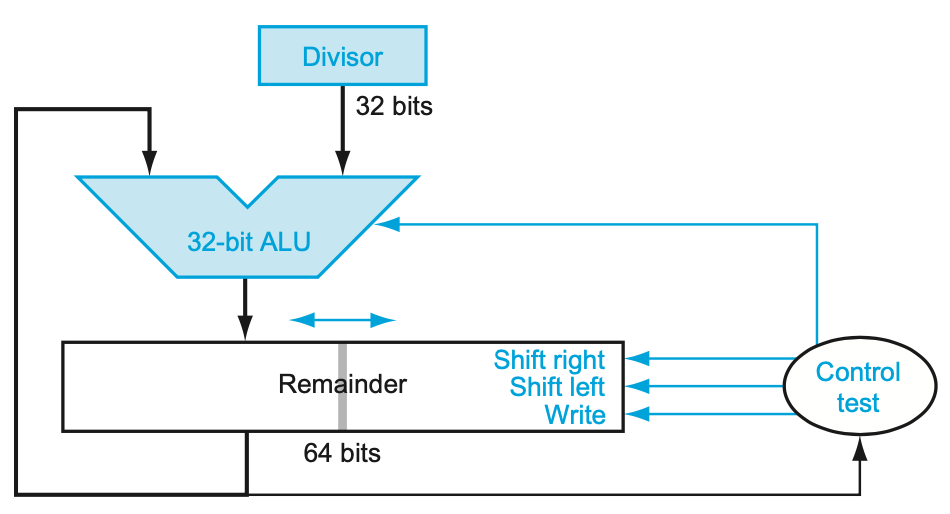
\includegraphics[width=7cm]{38.png}
  \caption{The faster division hardware}
  \label{fig:}
\end{figure}



\section{Basics of Logic Design}
For the most part we will be focusing on \textit{combinational logic}.  This is logic that has no memory (state) and therefore
\[\text{ Same Input } \Leftrightarrow   \text{ Same Output }.\]
\subsection{Truth Tables}\label{subsec:}
Because of the above fact, a combinational block can be completely described by a truth table. In a logic block an input is either true or false.  Therefore, a logic block with $n$ inputs has $2^n$ possible different possibilities.

Let's coonsider the logic function with inputs $(A,B)$ and outputs $(C,D,E)$ where:
\begin{itemize}
\item $C$ is true if no inputs are true,
\item $D$ is true if at least on input is true, and
\item $E$ is true if all inputs are true.
\end{itemize}
The truth table would be defined as follows
\[
\begin{tabular}{|c|c|c|c|c|}
\hline \multicolumn{2}{|c|}{ Inputs } & \multicolumn{3}{c|}{ Outputs } \\
\hline$A$ & $B$ & $C$ & $D$ & $E$ \\
  \hline \cellcolor{red!25}0 & \cellcolor{red!25}0 &  \cellcolor{green!25}1 & \cellcolor{red!25}0 & \cellcolor{red!25}0 \\
\hline \cellcolor{red!25}0 & \cellcolor{green!25}1 &  \cellcolor{red!25}0 & \cellcolor{green!25}1 & \cellcolor{green!25}1 \\
\hline \cellcolor{green!25}1 & \cellcolor{red!25}0 &  \cellcolor{red!25}0 & \cellcolor{green!25}1 & \cellcolor{red!25}0 \\
\hline \cellcolor{green!25}1 & \cellcolor{green!25}1 &  \cellcolor{red!25}0 & \cellcolor{green!25}1 & \cellcolor{green!25}1 \\
\hline
\end{tabular}.
\]
Sometimes truth tables are hard to read, so we can express each output of the truth table as a boolean expression:
\begin{align*}
  C &= \bar{A} \cdot \bar{B}\\
  D &= A + B\\
  E &= A \cdot B.
\end{align*}

\subsection{Boolean Algebra}\label{subsec:}
There are three elementary operators:
\begin{itemize}
\item logical OR: $A + B$,
\item logical AND: $A \cdot B$, and 
\item logical NOT: $\bar{A}$.
\end{itemize}
\subsubsection{Laws}
\begin{align*}
  \text{ Identity Laws: } A + 0 &= A\\
  A \cdot 1 &= A\\
  \text{ Zero and One Laws: } A + 1 &= 1\\
  A \cdot 0 &= 0\\
  \text{ Inverse Laws: } A + \bar{A} &= A\\
  A \cdot \bar{A} &= 0\\
  \text{ Commutative Laws: } A + B &= B + A\\
  A \cdot B &= B \cdot A\\
  \text{ Associative Laws: } A + (B + C) &= (A + B) + C\\
  A \cdot (B \cdot C) &= (A \cdot B) \cdot C\\
  \text{ Distributive Laws: } x \cdot(y + z)&=(x \cdot y) + (x \cdot z)\\
  \text{ DeMorgan's Laws: } \overline{(A + B)} &\Leftrightarrow \bar{A} \cdot \bar{B}\\
\overline{(A \cdot B)} &\Leftrightarrow \bar{A} + \bar{B}.
\end{align*}
\subsection{Logic Blocks}\label{subsec:}
We can implement truth tables and boolean expressions with the use of three types of logic gates:
\begin{align*}
\begin{circuitikz} \draw
  (0,0) node[and port] (and) {}
      (and.in 1) node [anchor=east] {A}
      (and.in 2) node [anchor=east] {B}
    \end{circuitikz} &&
\begin{circuitikz} \draw
  (0,0) node[or port] (or) {}
      (or.in 1) node [anchor=east] {A}
      (or.in 2) node [anchor=east] {B}
    \end{circuitikz} &&
\begin{circuitikz} \draw
  (0,0) node[not port] (not) {}
      (not.in 1) node [anchor=east] {A}
 \end{circuitikz}\\
  \text{ AND gate} && \text{ OR gate } && \text{ NOT gate}  
\end{align*}
For example, we can build function $C = \bar{A} \cdot \bar{B}$ as follows:
\begin{center}
\begin{circuitikz} \draw
  (0,0) node[not port] (not0) {}
      (not0.in 1) node [anchor=east] {B}
 (0,2) node[not port] (not1) {}
 (not1.in 1) node [anchor=east] {A}
 (2,1) node[and port] (and) {}
 (not0.out) -- (and.in 2)
 (not1.out) -- (and.in 1)
  (and.out) -- ++(0,0) node[right] {C}
    \end{circuitikz}
  \end{center}
  \subsubsection{Decoder}
  A decoder is a logic block that has $n$-bit input and $2^n$ outputs, where only one output is asserted for each input combination.  For example:
  
\[
\begin{tabular}{|c|c|c|c|c|c|}
\hline \multicolumn{2}{|c|}{ Inputs } & \multicolumn{4}{c|}{ Outputs } \\
\hline$A$ & $B$ & $C$ & $D$ & $E$ & F\\
 \hline \cellcolor{red!25}0 & \cellcolor{red!25}0 & \cellcolor{red!25}0 &  \cellcolor{red!25}0 & \cellcolor{red!25}0 & \cellcolor{green!25}1 \\
\hline \cellcolor{red!25}0 & \cellcolor{green!25}1 & \cellcolor{red!25}0 &  \cellcolor{red!25}0 & \cellcolor{green!25}1 & \cellcolor{red!25}0 \\
\hline \cellcolor{green!25}1 & \cellcolor{red!25}0 & \cellcolor{red!25}0 &  \cellcolor{green!25}1 & \cellcolor{red!25}0 & \cellcolor{red!25}0 \\
\hline \cellcolor{green!25}1 & \cellcolor{green!25}1 &  \cellcolor{green!25}1 & \cellcolor{red!25}0 & \cellcolor{red!25}0 & \cellcolor{red!25}0 \\
\hline
\end{tabular}.
  \]
  \begin{marginfigure}
    \begin{center}
      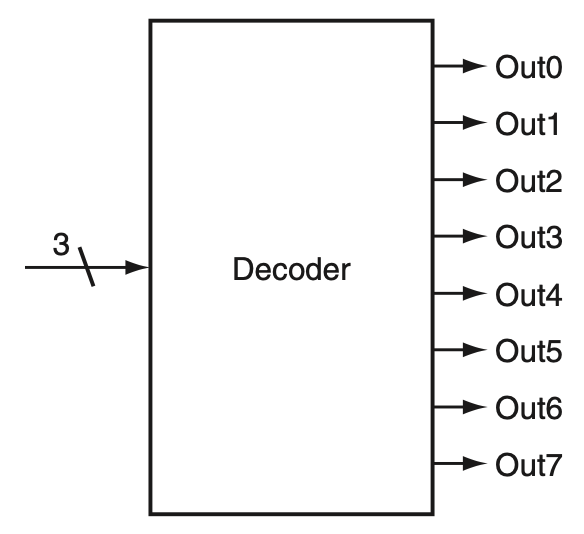
\includegraphics[width=\linewidth]{25.png}
    \end{center}
    \caption{A 3 bit decoder}
  \end{marginfigure}%

\subsubsection{Multiplexer}
  A multiplexer is selects one of the given inputs based upon the select signal given. A multiplexer has three parts:
  \begin{enumerate}
  \item A decoder that generates $n$ signals (from $\log_2 n$ inputs), each indicating a different input value
  \item An array of $n$ AND gates, each combining one of the inputs with a signal from the decoder
  \item A signle large OR gate that incorporates the outputs of the AND gates.  
  \end{enumerate}
\begin{figure}[H]
  \centering
  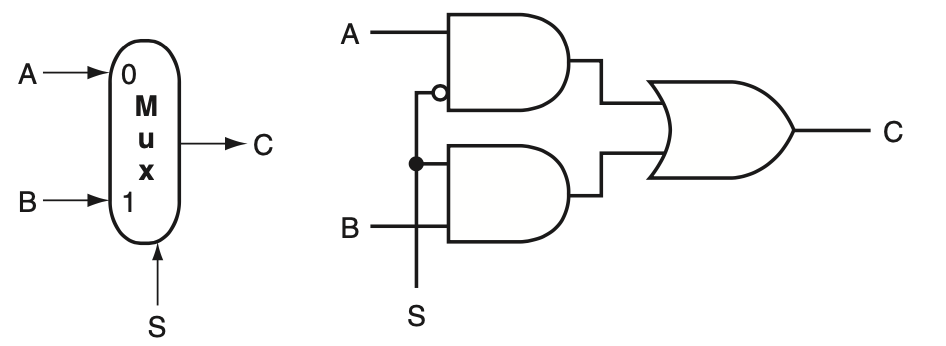
\includegraphics[width=7cm]{26.png}
  \caption{We can see either $A$ or $B$ is seleted based upon if the value of $S$ is $0$ or $1$.}
  \label{fig:}
\end{figure}
  The truth table for the above MUX will be
 \begin{center}
\begin{tabular}{|c|c|c|}
\hline index & $S$ & $C$ \\
 \hline 0 & \cellcolor{red!25}0 & $A$ \\
\hline 1 & \cellcolor{green!25}1 & $B$ \\
\hline
\end{tabular}, 
 \end{center} 
  and in boolean algebra:
  \[C = (\bar{S} \cdot A) + (S \cdot B).\]

\subsubsection{Two-Level Logic}
  Any logic function can be written where every \textbf{input} is either true or a complemented variable and there are only two levels of gates:
  \begin{itemize}
  \item an AND level and
  \item an or level.
  \end{itemize}
  There may be a possible inversion of the final output.  This is a lot to unpack, so let's look at an example.

  Let's say we are given the following truth table for $D$:
\begin{center}
\begin{tabular}{|c|c|c|c|c|c|}
  \hline \multicolumn{3}{|c|}{ Inputs } & { Outputs } \\
  \hline $A$ & $B$ & $C$ & $D$ \\
  \hline \cellcolor{red!25}0 & \cellcolor{red!25}0 & \cellcolor{red!25}0 &  \cellcolor{red!25}0 \\
  \hline \cellcolor{red!25}0 & \cellcolor{red!25}0 & \cellcolor{green!25}1 &  \cellcolor{green!25}1 \\
  \hline \cellcolor{red!25}0 & \cellcolor{green!25}1 & \cellcolor{red!25}0 &  \cellcolor{green!25}1 \\
  \hline \cellcolor{red!25}0 & \cellcolor{green!25}1 & \cellcolor{green!25}1 &  \cellcolor{red!25}0 \\
  \hline \cellcolor{green!25}1 & \cellcolor{red!25}0 & \cellcolor{red!25}0 &  \cellcolor{green!25}1 \\
  \hline \cellcolor{green!25}1 & \cellcolor{red!25}0 & \cellcolor{green!25}1 &  \cellcolor{red!25}0 \\
  \hline \cellcolor{green!25}1 & \cellcolor{green!25}1 & \cellcolor{red!25}0 &  \cellcolor{red!25}0 \\
  \hline \cellcolor{green!25}1 & \cellcolor{green!25}1 & \cellcolor{green!25}1 &  \cellcolor{green!25}1 \\
  \hline
\end{tabular}.
\end{center}
  Notice that there are four input combinations for which $D$ is true:
  \begin{marginfigure}
    A \textbf{product term} or a \textbf{minterm} is a set of logical inputs joined by conjunction (AND operations); the product terms for the first logic stage of the PLA.
  \end{marginfigure}%
\begin{itemize}
\item $\bar{A} \cdot \bar{B} \cdot C$
\item $\bar{A} \cdot B \cdot \bar{C}$
\item $A \cdot \bar{B} \cdot \bar{C}$
\item $A \cdot B \cdot C$
\end{itemize}
  We call each of these terms a \textbf{product term}.  For example the function $D$ can be implemented in hardware using two-level logic as follows:
\begin{center}
  \begin{circuitikz} \draw
    (0,0) node[and port] (and1) {}
    (0,2) node[and port] (and2) {}
    (0,4) node[and port] (and3) {}
    (0,6) node[and port] (and4) {}
    (4,3) node[or port, number inputs=4] (or) {}
    (and3.out) -- (or.in 2)
    (and2.out) -- (or.in 3)
    (and1.out) -- (or.in 4)
    (and4.out) -- (or.in 1)
    (or.out) -- ++(0,0) node[right] {D}
  \end{circuitikz}
\end{center}
  \subsubsection{Programmable Logic Array}
  When dealing with a set of logic functions (multiple inputs and multiple outputs) there will be an
  \begin{itemize}
  \item AND gate for each unique set of inputs for which there is at lest one corresponding true output
  \item OR gate for each output function.
  \end{itemize}
  This way of structured-logic implementation is called a programmable logic array.  Let's say we have the following logic table:
  \begin{center}
\begin{tabular}{|c|c|c|c|c|c|}
  \hline \multicolumn{3}{|c|}{ Inputs } & \multicolumn{3}{|c|}{ Outputs } \\
  \hline $A$ & $B$ & $C$ & $D$ & $E$ & $F$\\
  \hline \cellcolor{red!25}0   & \cellcolor{red!25}0   & \cellcolor{red!25}0   &  \cellcolor{red!25}0   & \cellcolor{red!25}0   & \cellcolor{red!25}0     \\
  \hline \cellcolor{red!25}0   & \cellcolor{red!25}0   & \cellcolor{green!25}1 &  \cellcolor{green!25}1 & \cellcolor{red!25}0   & \cellcolor{red!25}0  \\
  \hline \cellcolor{red!25}0   & \cellcolor{green!25}1 & \cellcolor{red!25}0   &  \cellcolor{green!25}1 & \cellcolor{red!25}0   & \cellcolor{red!25}0  \\
  \hline \cellcolor{red!25}0   & \cellcolor{green!25}1 & \cellcolor{green!25}1 &  \cellcolor{green!25}1 & \cellcolor{green!25}1 & \cellcolor{red!25}0  \\
  \hline \cellcolor{green!25}1 & \cellcolor{red!25}0   & \cellcolor{red!25}0   &  \cellcolor{green!25}1 & \cellcolor{red!25}0   & \cellcolor{red!25}0  \\
  \hline \cellcolor{green!25}1 & \cellcolor{red!25}0   & \cellcolor{green!25}1 &  \cellcolor{green!25}1 & \cellcolor{green!25}1 & \cellcolor{red!25}0  \\
  \hline \cellcolor{green!25}1 & \cellcolor{green!25}1 & \cellcolor{red!25}0   &  \cellcolor{green!25}1 & \cellcolor{green!25}1 & \cellcolor{red!25}0  \\
  \hline \cellcolor{green!25}1 & \cellcolor{green!25}1 & \cellcolor{green!25}1 &  \cellcolor{green!25}1 & \cellcolor{red!25}0   & \cellcolor{green!25}1  \\
  \hline
\end{tabular}.
\end{center}
  Then the associated PLA that implements the logic function is:
\begin{figure}[H]
  \centering
  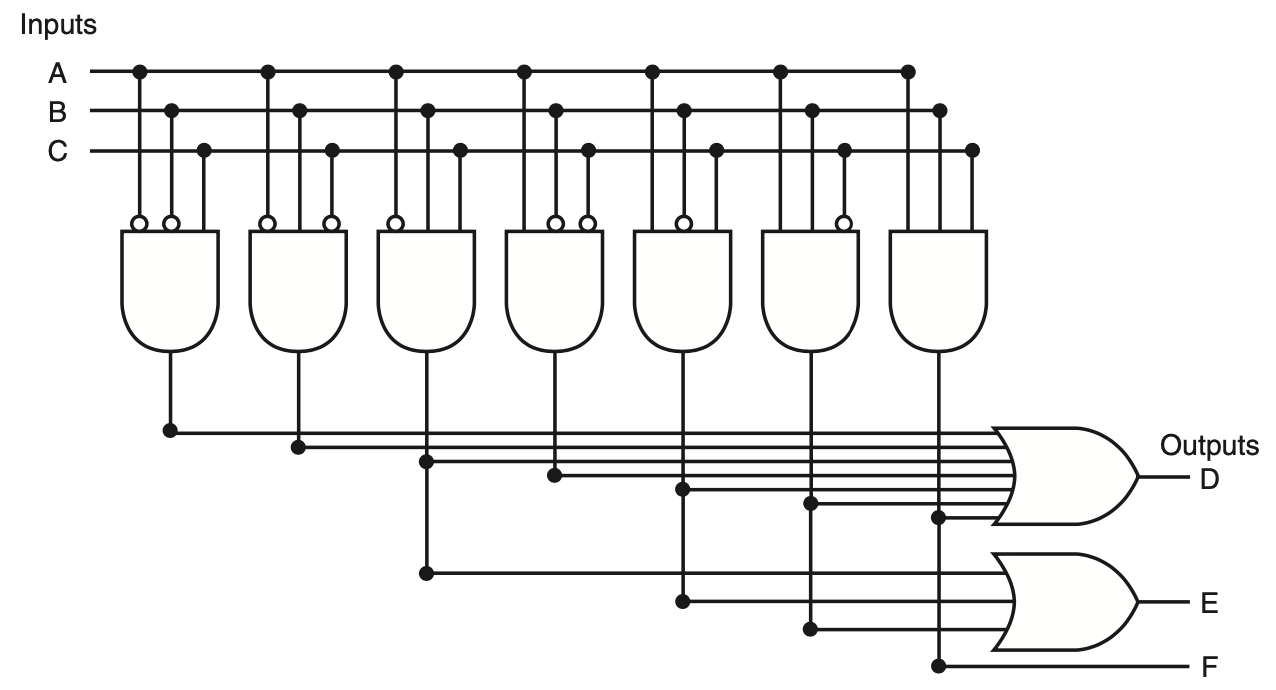
\includegraphics[width=9cm]{27.png}
  \caption{Notice that only $7$ AND gates are required because no function is true for $A = B = C = 0$, and so we can ignore that. Also note that although there are three functions, there are only two OR gates because only combination of inputs for turns $F$ on.}
    \label{fig:}
  \end{figure}

\subsubsection{Don't Cares}
  Don't cares, as the name suggests, are values of an input, or values of an output for which we don't care what the value is; the value could be either $0$ or $1$ and the effect of the logic block would be unchanged.  
  \begin{itemize}
  \item Input Don't Cares: Arise when an output depends on only some of the inputs
  \item Output Don't Cares: Arise when we don't care about the value of an output because another output is true.
\end{itemize}
    Don't cares are shown as X's on a truth table. They are important because they make it easeir to implement the optimization of a logic function. For example, consider the following logic functions:
    \begin{itemize}
    \item $D$ is true if $A$ or $C$ is true
    \item $E$ is true if $A$ or $B$ is true
    \item $F$ is true if exactly one of the inputs is true. But we don't care about $F$ if both $D$ and $E$ are true
    \end{itemize}
  The truth table is as follows:
  \begin{figure}[H]
    \centering
   \begin{tabular}{|c|c|c|c|c|c|}
  \hline \multicolumn{3}{|c|}{ Inputs } & \multicolumn{3}{|c|}{ Outputs } \\
  \hline $A$ & $B$ & $C$ & $D$ & $E$ & $F$\\
  \hline \cellcolor{red!25}0   & \cellcolor{red!25}0   & \cellcolor{red!25}0   &  \cellcolor{red!25}0   & \cellcolor{red!25}0   & \cellcolor{red!25}0     \\
  \hline \cellcolor{red!25}0   & \cellcolor{red!25}0   & \cellcolor{green!25}1 &  \cellcolor{green!25}1 & \cellcolor{red!25}0   & \cellcolor{green!25}1\\
  \hline \cellcolor{red!25}0   & \cellcolor{green!25}1 & \cellcolor{red!25}0   &  \cellcolor{red!25}0   & \cellcolor{green!25}1 & \cellcolor{green!25}1  \\
  \hline \cellcolor{red!25}0   & \cellcolor{green!25}1 & \cellcolor{green!25}1 &  \cellcolor{green!25}1 & \cellcolor{green!25}1 & \cellcolor{red!25}0  \\
  \hline \cellcolor{green!25}1 & \cellcolor{red!25}0   & \cellcolor{red!25}0   &  \cellcolor{green!25}1 & \cellcolor{green!25}1   & \cellcolor{green!25}1  \\
  \hline \cellcolor{green!25}1 & \cellcolor{red!25}0   & \cellcolor{green!25}1 &  \cellcolor{green!25}1 & \cellcolor{green!25}1 & \cellcolor{red!25}0  \\
  \hline \cellcolor{green!25}1 & \cellcolor{green!25}1 & \cellcolor{red!25}0   &  \cellcolor{green!25}1 & \cellcolor{green!25}1 & \cellcolor{red!25}0  \\
  \hline \cellcolor{green!25}1 & \cellcolor{green!25}1 & \cellcolor{green!25}1 &  \cellcolor{green!25}1 & \cellcolor{green!25}1   & \cellcolor{red!25}0  \\
  \hline
\end{tabular}.
\begin{tabular}{|c|c|c|c|c|c|}
  \hline \multicolumn{3}{|c|}{ Inputs } & \multicolumn{3}{|c|}{ Outputs } \\
  \hline $A$ & $B$ & $C$ & $D$ & $E$ & $F$\\
  \hline \cellcolor{red!25}0   & \cellcolor{red!25}0   & \cellcolor{red!25}0   &  \cellcolor{red!25}0   & \cellcolor{red!25}0   & \cellcolor{red!25}0     \\
  \hline \cellcolor{red!25}0   & \cellcolor{red!25}0   & \cellcolor{green!25}1 &  \cellcolor{green!25}1 & \cellcolor{red!25}0   & \cellcolor{green!25}1\\
  \hline \cellcolor{red!25}0   & \cellcolor{green!25}1 & \cellcolor{red!25}0   &  \cellcolor{red!25}0   & \cellcolor{green!25}1 & \cellcolor{green!25}1  \\
  \hline \cellcolor{blue!25}X  & \cellcolor{green!25}1 & \cellcolor{green!25}1 &  \cellcolor{green!25}1 & \cellcolor{green!25}1 & \cellcolor{blue!25}X  \\
  \hline \cellcolor{green!25}1 & \cellcolor{blue!25}X  & \cellcolor{blue!25}X  &  \cellcolor{green!25}1 & \cellcolor{green!25}1 & \cellcolor{blue!25}X  \\
  \hline
\end{tabular}.
    \caption{Notice that with the use of don't cares, we can have the truth table be smaller because of repeated rows.}
    \label{fig:}
  \end{figure}
\subsubsection{Arrays of Logic Units}
  Up until now we have been performing combinational operations on just single bits, but we often want to do the same operations on whole words ($32$-bits).  For example you may want to see if the value in one register is the same as the value as the other.  Or you may want to have a MUX that selects between two words, and not just two bits:
  \begin{figure}[H]
    \centering
    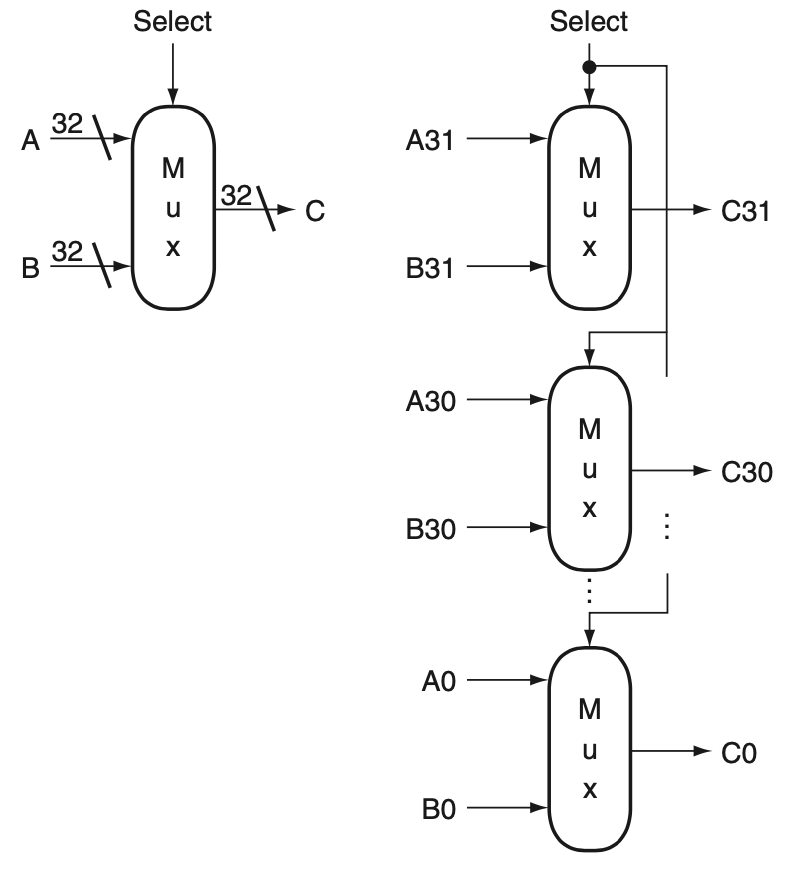
\includegraphics[width=9cm]{28.png}
    \caption{The $32$-bit MUX is just $32$ 1-bit MUX's connected together.}
    \label{fig:}
  \end{figure}

  \section{Constructing a Basic Arithmetic Logic Unit}
An ALU is the part of the processor that is responsible for performing both logical and arithmetic operations such as addition, subtraction, AND, and OR.
\subsection{1-Bit ALU}\label{subsec:}
  Let's go about implementing each of the different operations an ALU can perform.
  \subsubsection{AND / OR Logical Operation}
  To implement this you just have a MUX that selects between the AND, and OR operations:
  \begin{figure}[H]
    \centering
    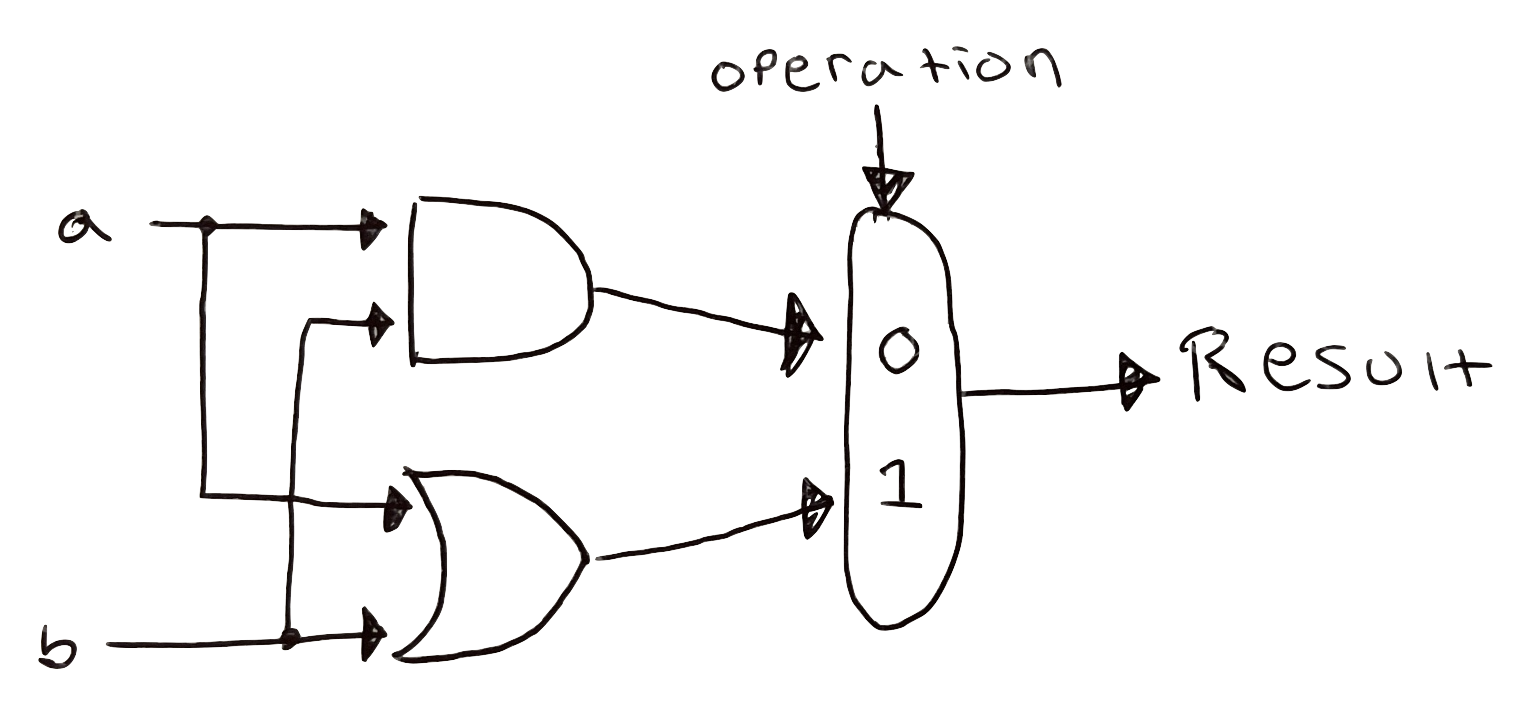
\includegraphics[width=8cm]{30.png}
    \caption{The multiplexor selects between and or or depending upon the opcode recieved.}
    \label{fig:}
  \end{figure}

  \subsubsection{Addition}
  To implement addition, with each bit in addition to looking at the bits adding together we also want to see if there was carryover from the the prior (less significant) bit.  Thus, to deploy our operation in hardware we will need three \textbf{inputs}:
  \begin{itemize}
  \item $a$
  \item $b$
  \item carry in
  \end{itemize}
  and two \textbf{outputs}:
  \begin{itemize}
  \item computed sum
  \item carry out.
  \end{itemize}
  How is the carry out computed?  Well, there is carry out if 2 or 3 of the inputs are true.  Thus we have
  \begin{align*}
\text{ Carry Out } &= (a \cdot b) + (a \cdot \text{ carry in}) + (b \cdot \text{ carry in})
                     + (a\cdot b \cdot \text{ carry in})\\
                   &=  (a \cdot b) + (a \cdot \text{ carry in}) + (b \cdot \text{ carry in}).
  \end{align*}
  Implementing this using logic gates we have:
  \begin{figure}[H]
    \centering
    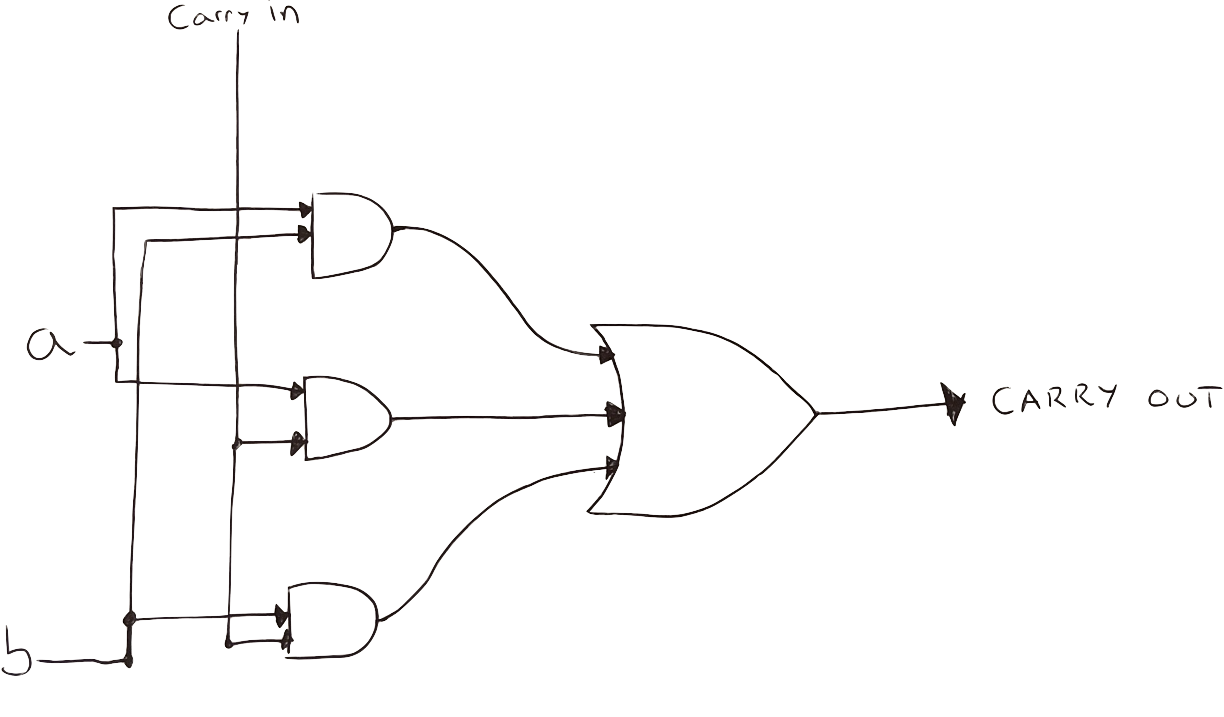
\includegraphics[width=8cm]{31.png}
    \caption{For cary out to be true we need to have t least two of the inputs to be true.}
    \label{fig:}
  \end{figure}
  To calculate the \textbf{sum} using logic we see that sum will be true if an odd number of inputs are true (1 or 3).  Therefore:
  \begin{align*}
    \text{ sum } &= (a \cdot \bar{b} \cdot \overline{\text{carry in}}) + (\bar{a} \cdot b \cdot \overline{\text{carry in}}) + (\bar{a} \cdot \bar{b} \cdot \text{  carry in}) + (a\cdot b \cdot \text{ carry in}). 
  \end{align*}
  Implementing this using logic gates we have:
\begin{figure}[H]
  \centering
  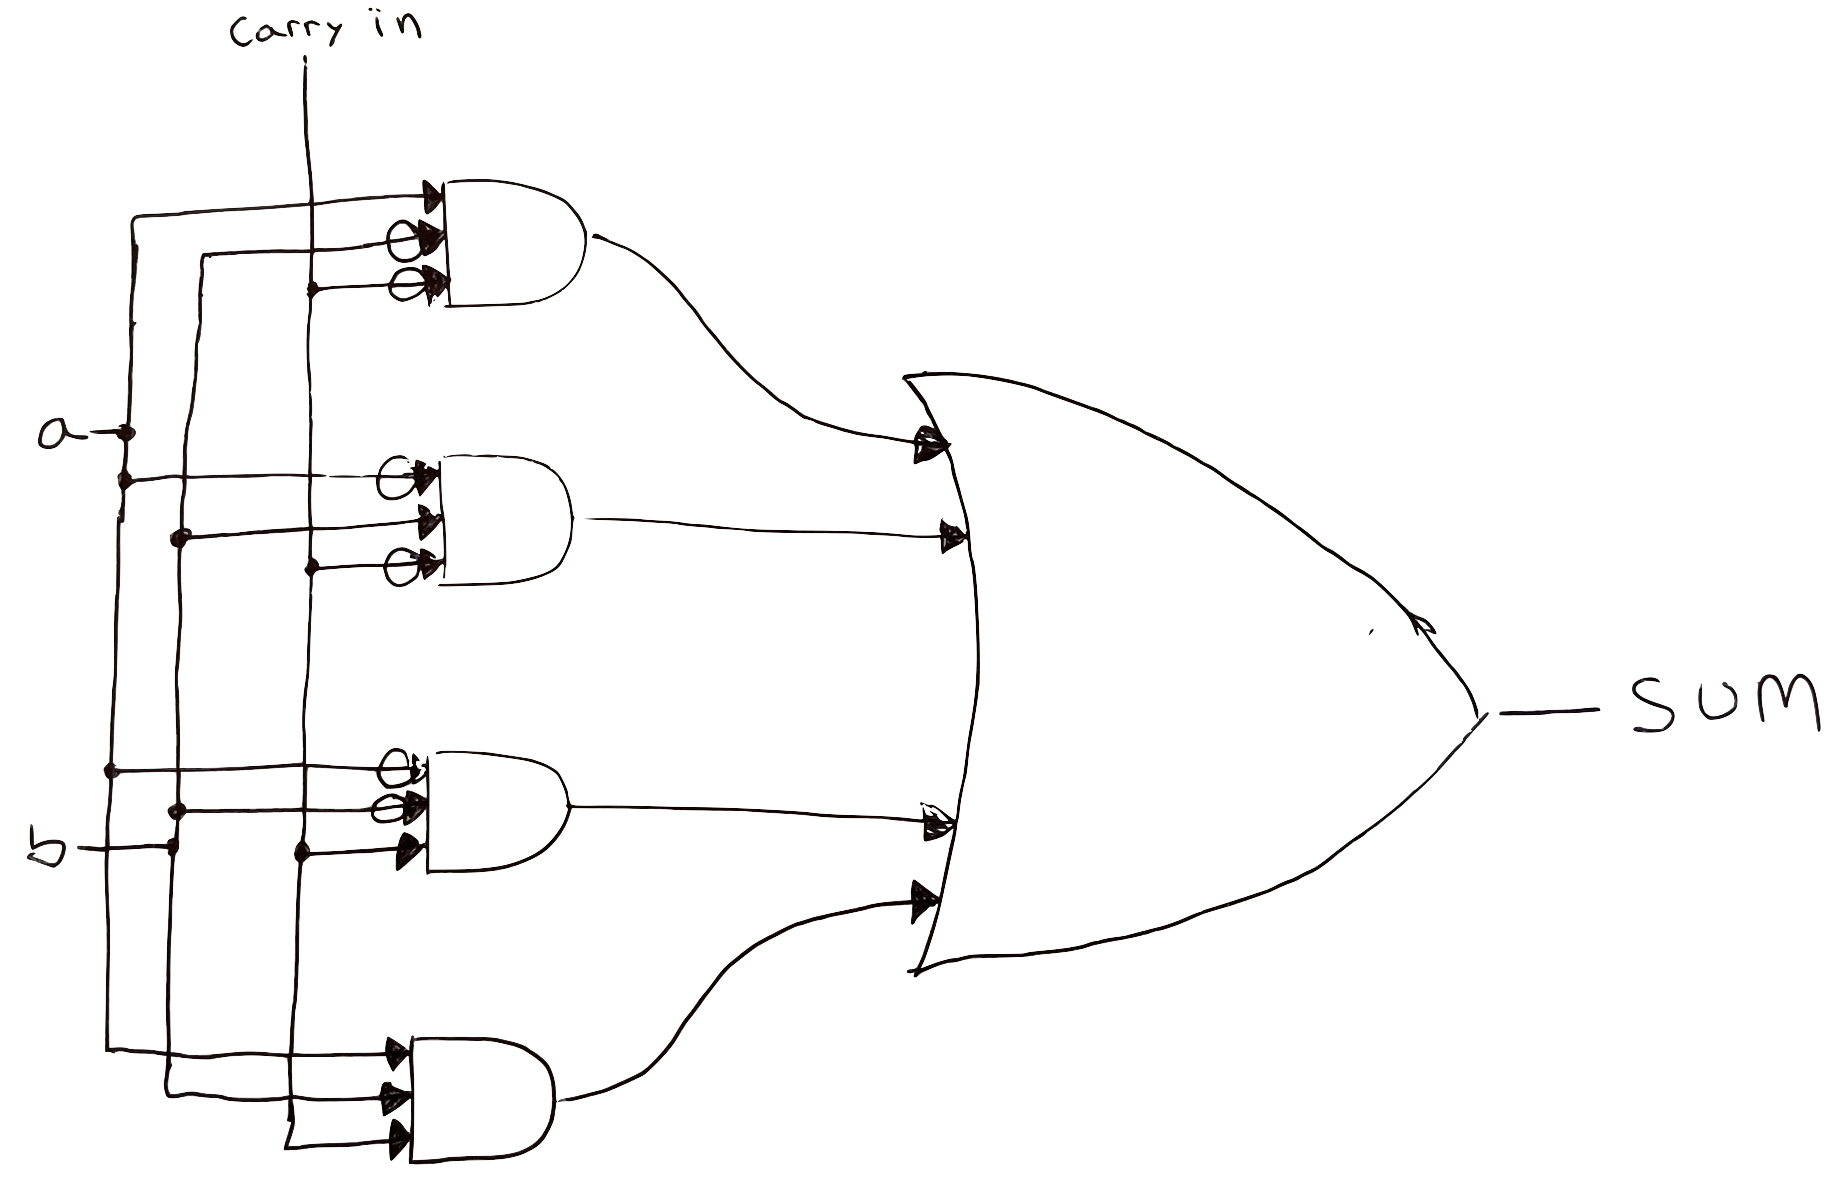
\includegraphics[width=8cm]{32.png}
  \caption{Sum is true if there are an odd number of true inputs.}
  \label{fig:}
\end{figure}
\subsubsection{Completing the 1-Bit ALU}
To complete the 1-bit ALU we just connect the AND/OR/ADD operations to a mux that selects the desired operation.

\subsection{32-Bit ALU}\label{subsec:}
The 32-bit ALU is created by connecting 32 1-bit ALU together.  Although we have our 1-bit ALU, there are some additional features that we want to make sure we have.
\subsubsection{Subtraction}
To compute subtraction we will use the addition we have already implemented and add a negative number.  We can do this because $-b = \bar{b} + 1$.  To get $\bar{x}$ we thus need an inverter that inverts each of the bits of $b$.  We need to connect that inverter to a MUX which selects the inverted $b$ (if subtraction) or the original $b$ (if addition). We will add one through the use of the carry in input of the lsb since that will be $0$ when addition and $1$ when subtraction.
\begin{figure}[H]
  \centering
  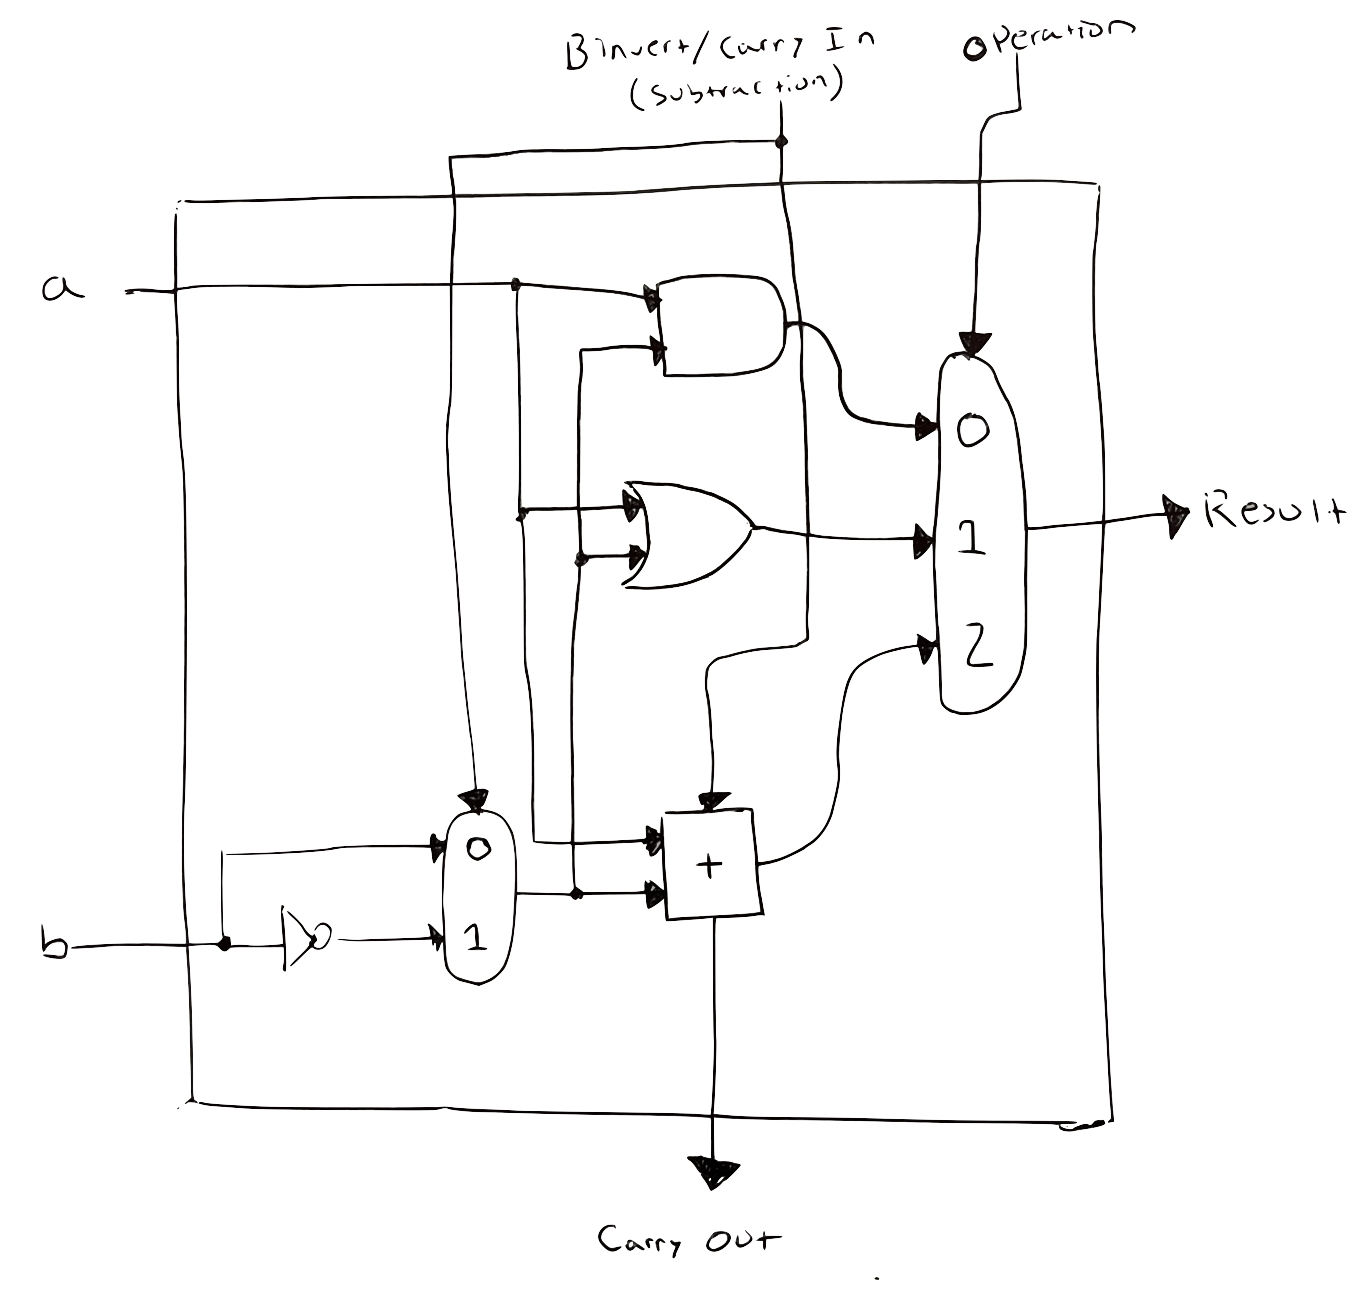
\includegraphics[width=6cm]{33.png}
  \caption{For subtraction we use the value of carry in to additionally select whether we should invert $b$ or not.  The operation code selects between AND, OR, and ADD (which also performs subtraction depending upon value of carry in).}
  \label{fig:}
\end{figure}

\subsubsection{NOR (Neither a nor b)}
Because
\[(\overline{a + b}) = \bar{a} \cdot \bar{b}\]
we are able to utilize the existing Binvert and AND gate and only need to add an inversion of a.
\begin{figure}[H]
  \centering
  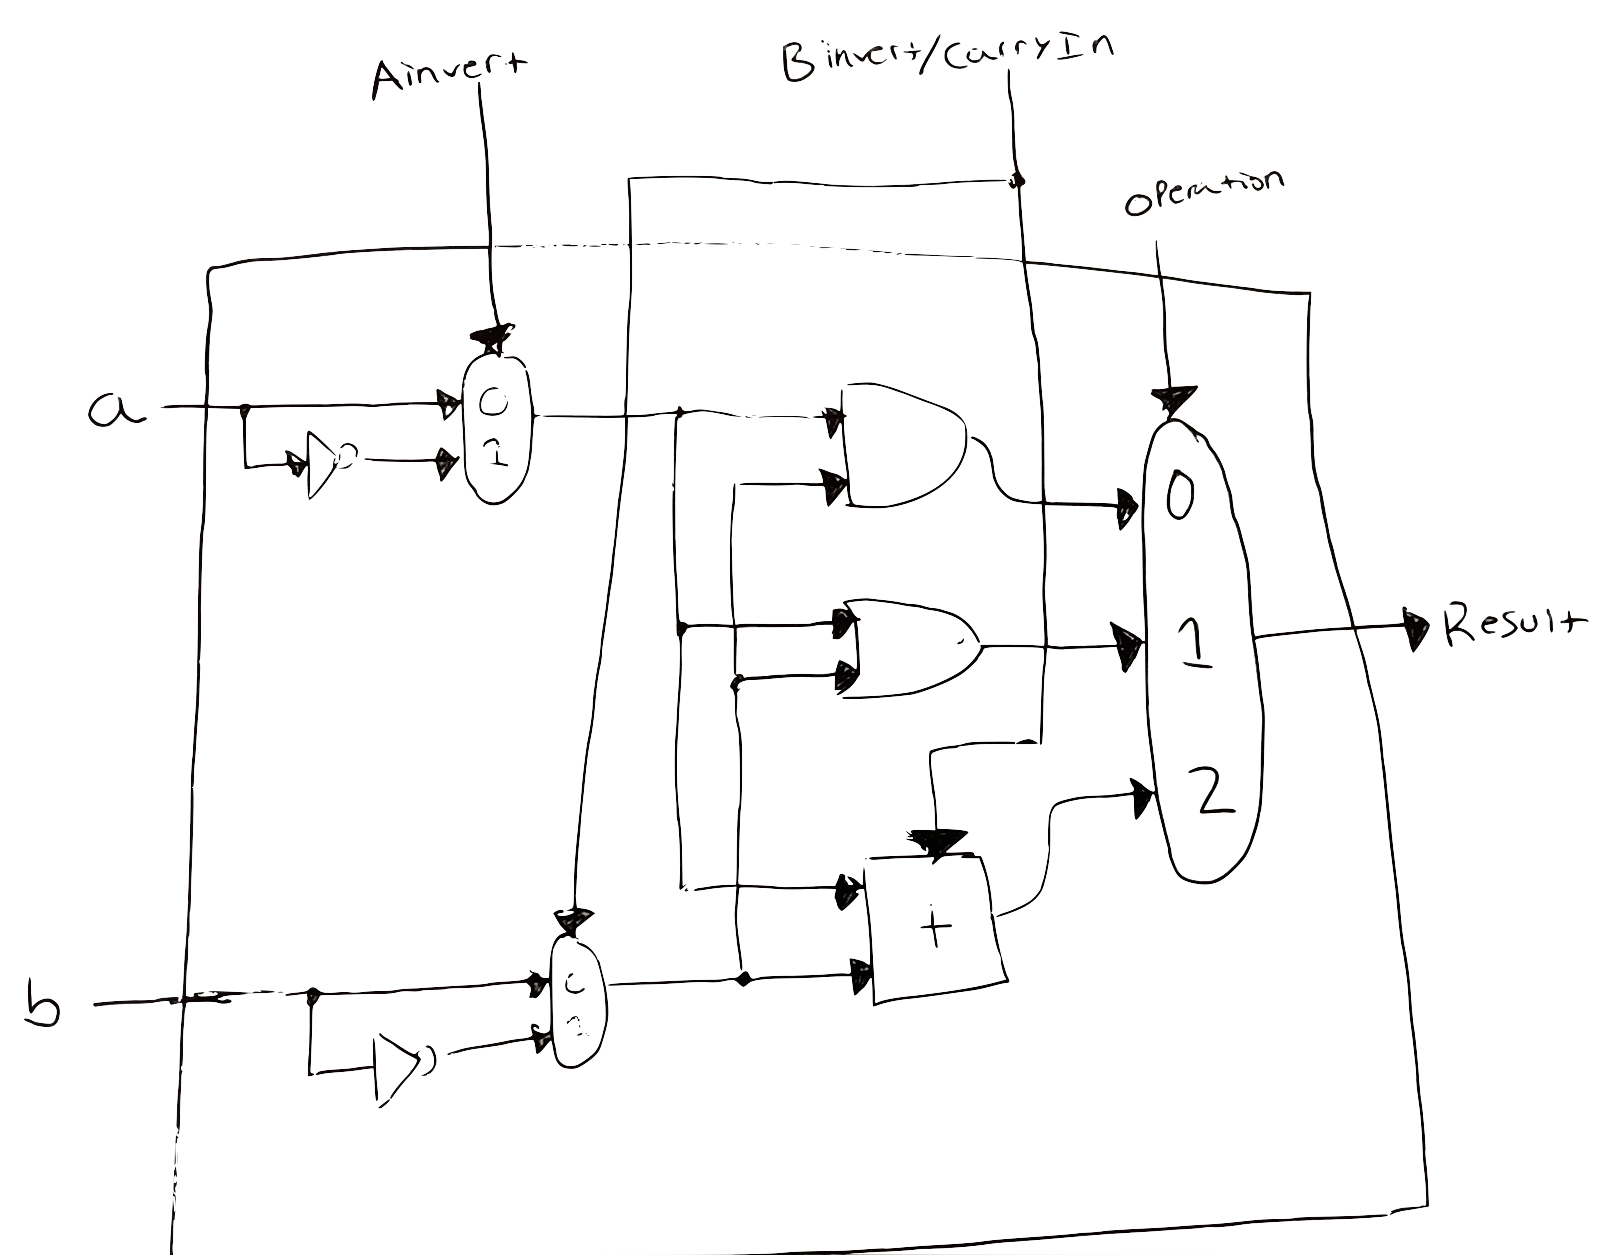
\includegraphics[width=8cm]{34.png}
  \caption{For NOR the output of the AND gate is used but with both Ainvert and Binvert inputs set as true.}
  \label{fig:}
\end{figure}
\pagebreak
\subsubsection{Shift Less Than}
For \texttt{slt} we return $1$ if \texttt{rs < rt} and $0$ otherwise.  To test for this we can use subtraction because
\[a < b \Leftrightarrow (a-b) < 0\]
and thus if the result of $a-b$ is negative we set the lsb to 1.  How does this work in practice?  Well the 31 most significant ALUs are easy, we just connect 0 directly to the MUX that selects the desired operation. We will label this input \texttt{sltResult}.  For the least significant bit we connect the result of the adder of the msb to the least significant bit input \texttt{sltResult}.
\begin{figure}[H]
  \centering
  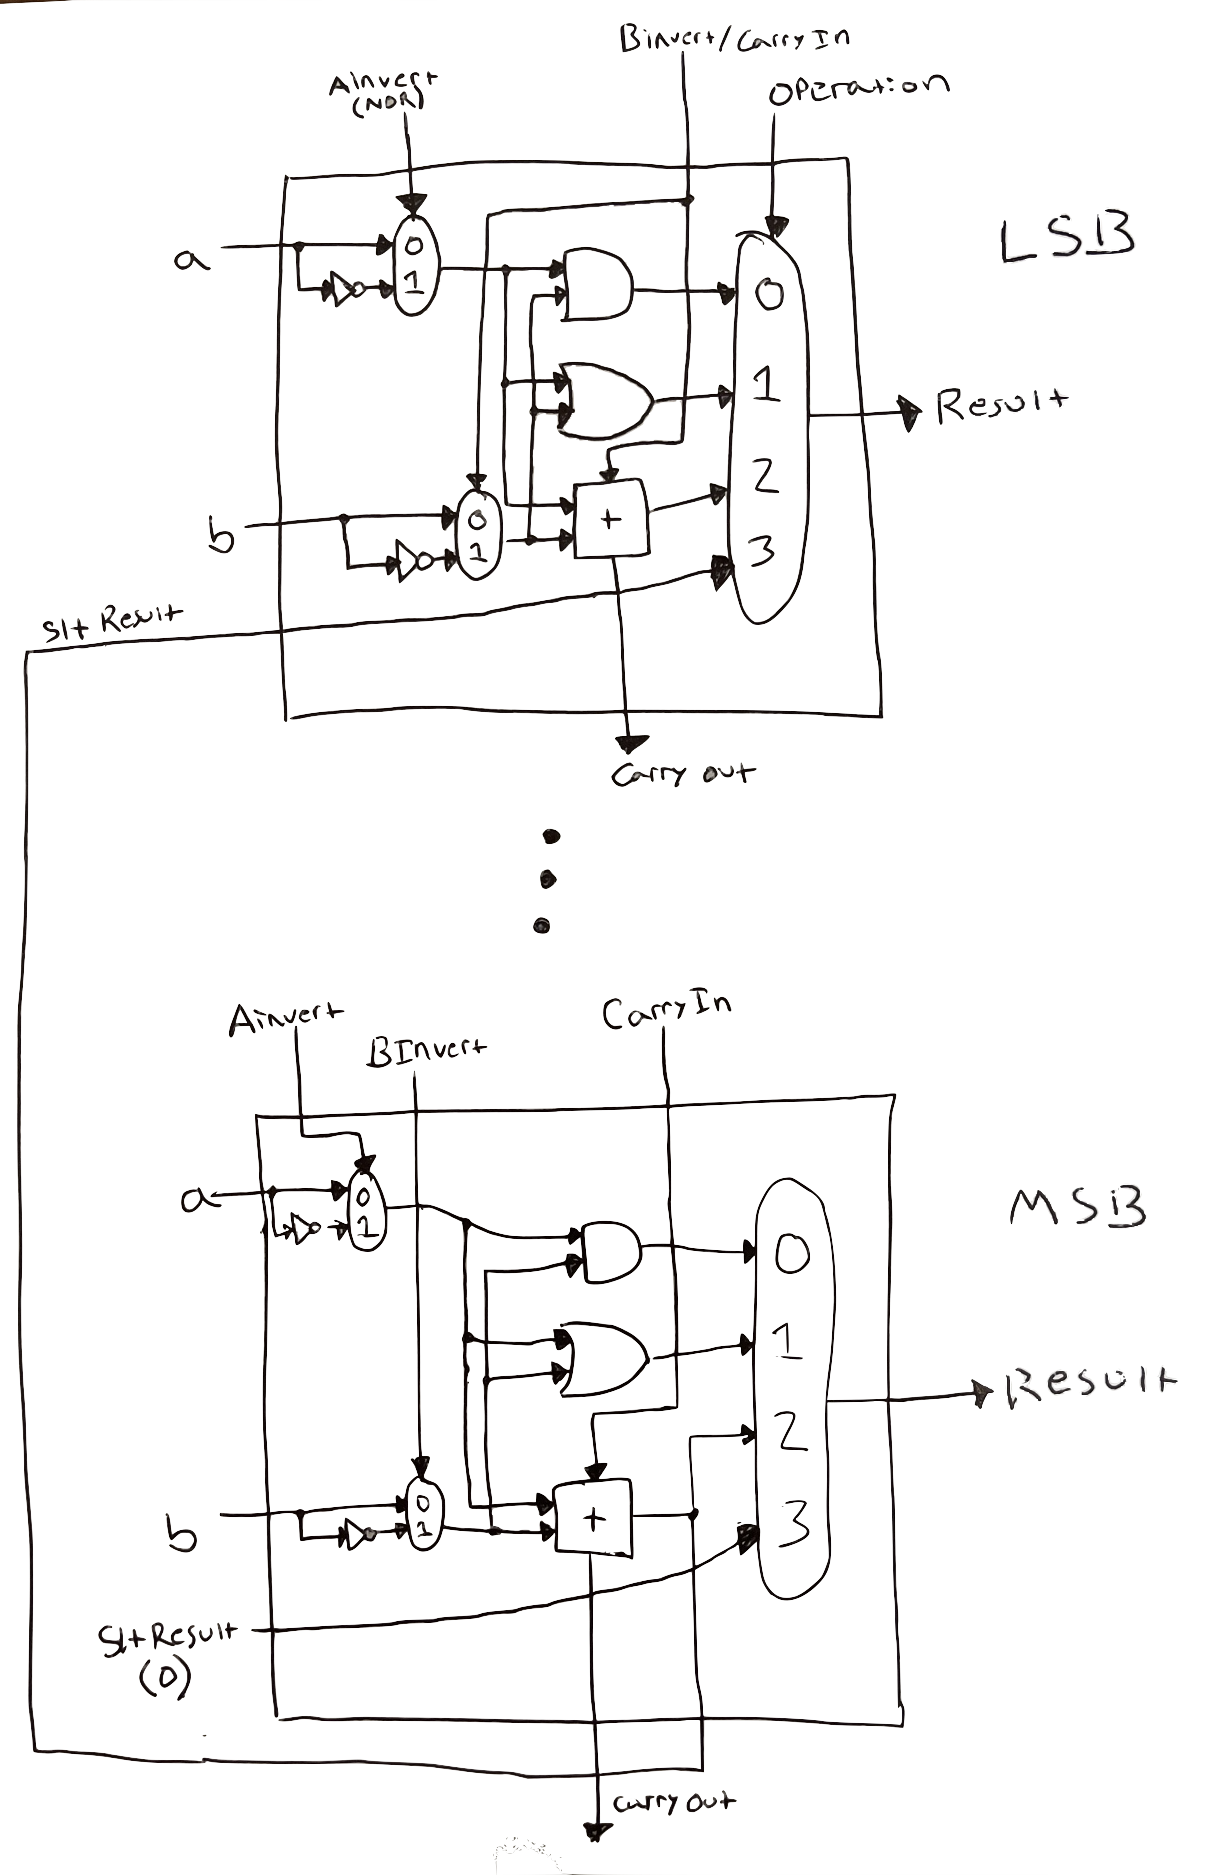
\includegraphics[width=8cm]{35.png}
  \caption{To perform \texttt{slt} we set operation to 3, Binvert to $1$ and \texttt{sltResult} to 0 for the 31 MSBs but use the result of the adder for the MSB to set the value of \texttt{sltResult} of the LSB}
  \label{fig:}
\end{figure}





\end{document}
      